% !TEX program = pdflatex
% !TEX enableSynctex = true
% !BIB program = bibtex

\documentclass[12pt]{article}

\usepackage{setspace}
\usepackage{amsmath}
\usepackage{amsfonts}
\usepackage{graphicx}
\usepackage{float}
\usepackage{dsfont}
\usepackage{natbib}
\addtolength{\oddsidemargin}{-.7in}
\addtolength{\evensidemargin}{-.7in}
\addtolength{\textwidth}{1.4in}
\usepackage{enumerate}
\onehalfspacing
\usepackage{geometry} % Required for customizing page layout
\usepackage{ragged2e}

\usepackage{caption}
\usepackage{booktabs}

\usepackage{hyperref}
\hypersetup{
	pdfstartview = FitH,
	pdfauthor = {...},
	pdftitle = {...},
	pdfkeywords = {...; ...; ...; ...},
	colorlinks = true,
	linkcolor = blue,
	urlcolor = blue,
	citecolor = blue,
	linktocpage=true
}

\DeclareMathOperator{\E}{\mathbb{E}}
\DeclareMathOperator*{\argmax}{arg\,max}
\DeclareMathOperator*{\argmin}{arg\,min}

\title{Credit Spreads, Liquidation Probability and Access to Cash Flow-Based debt}
\date{}

\begin{document}

\author{Barnabás Székely}
\date{\today}
\vspace{-1in}

\maketitle

\begin{abstract}
\noindent

I study the credit spreads of asset-based and cash flow-based debt contracts in a heterogeneous firms model with in-equilibrium defaults. For CF-based debt contracts, an important yet under-studied determinant is the ex-ante probability that the firm would be liquidated under financial distress. This puts small businesses, which often choose liquidation, at a disadvantage. Their access to cash flow-backed debt is limited by high ex-ante liquidation probabilities, whereas their access to asset-based debt is constrained by a lack of pledgeable assets. The structural model suggests that the resulting misallocation of capital yields significant productivity losses. However, this could be mitigated by cutting the reorganization costs. I find that reducing these costs to a quarter would boost aggregate productivity by 2.4\%. 

\bigskip{}
\bigskip{}
%\bigskip{}
%\bigskip{}
%\vspace{-0.5cm}

Keywords: Heterogeneous firms, Credit market frictions, Cash flow-based lending, Earnings-based constraints

\medskip{}
% JEL Classification Code: E32, C22, E27.
\end{abstract}
\thispagestyle{empty}

\pagebreak{}

\section{Introduction \label{sec:introduction}} 
Corporate credit market frictions are typically characterized as borrowing constraints defined the by value of pledgeable assets. Recent research has challenged this view based on more granular analyses of corporate credit contracts. These argue that the majority of corporate debt is backed by borrowers’ future cash flows rather than assets, which implies that credit frictions are better described as borrowing constraints defined by current earnings. These results led to several contributions focused on re-assessing credit market frictions in structural analyses. \vspace{3mm} \\
However, such studies typically adopt a `no equilibrium defaults' framework,\footnote{Dating back to Kiyotaki and Moore (1997).} where lenders impose borrowing limits to such that firms always meet their debt obligations. This gives rise to `hard constraints' to borrowing. Firms that borrow against assets are constrained by the value of their collateral, whereas those borrowing against cash flows are limited by current earnings. One shortcoming of this framework is its inability to account for variations of interest rates across firms - since debt contracts are always honored, every firm faces the same risk-free rate. This directed the focus of this literature to studying the effects of debt covenants,\footnote{These are legally binding agreements imposed by the creditor on the lender, that typically take the form of hard constraints implied by the no equilibrium defaults framework.} while credit spreads received considerably less attention.  \vspace*{3mm} \\
I fill this gap in the literature by studying the determinants of credit spreads for asset-based and cash flow-based debt. This requires a model framework where a certain proportion of firms choose to file for bankruptcy each period. Moreover, debt may be backed by assets, such that lenders' in-default payments are determined by their liquidation value, or by future cash flows, such that lenders' in-default payments reflect the going-concern value of the firm. Lenders set interest rates following their exposure to default and the probability of this event. Both of these increase with debt, causing interest rates to rise with borrowing. This yields `soft borrowing constraints', specific to firms' current state, credit demand and debt financing strategy, which allows me the structural analysis of credit spreads while considering heterogeneity in debt contracts. \vspace*{3mm} \\
\textbf{Here, mention the empirical analysis and find a segway to the importance of the liquidation probability} The structural model is supported by an empirical analysis of debt US debt contracts between 2010-2023. For both type of debt, I observe a negative relationship between credit spreads and the probability of liquidation, as well as assets. This finding contradicts the predictions of `hard constraints framework' as it suggests that size and profitability are important determinants of credit market frictions regardless of the type of borrowing. \vspace{3mm} \\
Bankrupt firms may undergo liquidation or reorganization (Chapter 7 and Chapter 11 in the US bankruptcy code). In the absence of collateral, the lender may retrieve only a fraction of the borrower's liquidation value. Hence, CF-based debt is backed mainly by the belief that the borrower would produce positive cash-flows even after experiencing financial distress. Choosing liquidation in bankruptcy terminates all future cash-flows. \textit{This turns the lending problem, into commitment issue.} \vspace{3mm} \\
Hence, high ex-ante probability of liquidation raises the credit spread of CF-based debt, by increasing lenders' exposure to default. Crucially, the proportion of liquidating firms decreases sharply with size. For instance, 56.6\% of firms with less than 100 million USD worth of total assets liquidate, but only 4.27\% of firms larger than this do so. I argue that in the case of CF-based debt, the value of assets serves as a proxy of liquidation probability rather than a direct determinant of in-default payments. \vspace*{3mm} \\ 
To study the impact of this trend, I consider endogenous liquidation decision in structural the model, similar to Corbae and D'Erasmo (2021). Firms in financial distress may  be liquidated, which entails exiting the market, or reorganized, which allows them to continue but incurs significant fixed costs.\footnote{These are generated by the time, legal and personnel expenses involving the renegotiation of debt \textit(cit).} This introduces economies of scale in reorganizations. Small firms are at a disadvantage under both type of debt contracts. Their access to CF-based debt is limited by high liquidation probabilities, while their access to asset based debt is limited by the amount of pledgeable assets. The model suggest that these compounding disadvantages are an important source of capital misallocation. However, bankruptcy framework that incentivise and facilitate small firm reorganization can mitigate this effect. \vspace*{3mm} \\
The paper is organized as follows. Section 2 reviews the related literature. Section 3 addresses the empirical analysis, beginning with a description of the data and the classification of debt contracts into asset-based and cash flow-based. It then presents descriptive statistics for debt contracts and firm characteristics. Lastly, it analyzes the empirical predictors of credit spreads and debt financing strategies. Section 4 introduces the structural model and section 5 discusses the results. Section 6 concludes.

\section{Literature \label{sec:literature}} 
This ppaper reflects on the contributions the highlight the prevalence of CF-based borrowin. Lian and Ma (2021) finds that majority of US corporate debt is backed by future cash flows rather than specific physical assets, which suggests that credit frictions are better described as earnings-based constraints. They support this finding by documenting the extensive use of earnings-based covenants in US corporate debt contracts. Similarly, Drechsel (2023) finds that three of the four most frequently used debt covenants limit debt based on current earnings rather than assets. \vspace{3mm} \\
These results led to the reevaluation credit frictions in macroeconomic models. Switching to earnings based constraints have been shown to have substantial impact on various model outcomes. Lian and Ma (2021) argues that this mitigates the financial acceleration driven by feedback of asset prices into credit constraints.\footnote{This mechanism was first highlighted by Bernanke, Gertler, and Gilchrist (1999).} Drechsel and Kim (2022) argues that firms subject to earnings based constraints under-borrow, while those facing asset based constraints over-borrow. Drechsel (2023) considers `investment shocks' that move the price of the capital countercyclically. He demonstrates that the effects of such shocks are heterogeneous depending on the borrowing constraint in place.  \vspace{3mm} \\
Earnings-based constraints have also been studied in relation to monetary policy, since unlike asset-based constraints, these directly interact with sticky prices. Greenwald (2019) points out interest coverage covenants, which limit borrowing in the ratio of interest payments to earnings introduce a direct channel of monetary policy transmission. Caglio, Darst and Kalemli-Ozcan (2021) studies the investment and credit channel of monetary policy when firms are backed by different type of collateral. They document that small and risky firms often rely on `going-concern value' collateral, which makes them more responsive to monetary policy shocks. \vspace{3mm} \\
The structural model proposed here adopts the heterogeneous firms framework established by Khan, Senga and Thomas (2013). This framework has been extended to study the decision to borrow against assets or cash flows. Öztürk (2023) highlights the volatility of earnings and pledgeability as important determinants of this decision. Gonzalez and Sy (2024) documents on Spanish data that reliance to CF-based borrowing (CF-based debt to total debt) is U-shaped across firms size, meaning that small and large firms borrow most against cash flows. On the other hand, empirical research such as Kermani and Ma (2020) highlight the importance of `asset specificity,' which describes how much value assets would lose under liquidation. \footnote{These papers are closely related to my research, since credit conditions and the debt financing strategy are jointly determined. Firms react to the credit conditions set by debt covenants and credit spreads by optimizing their debt financing strategy, which in turn affects the credit market frictions they eventually face.} \vspace{3mm} \\
Both Öztürk (2023) and Gonzalez and Sy (2024) adopt the `hard constraints' framework where firms choose between earnings-based or asset-based constraints based on which is less restrictive. In essence, this amounts to modelling heterogeneity in borrowing constraints. This approach does not allow for holding both types of debt simultaneously, which can be a significant limitation, since in the United States these borrowers represent a substantial share of the market. 
Conversely, I consider heterogeneity in debt contracts (differences in in-default payoffs) rather than borrowing constraints. This yields a more flexible framework that allows for firms that hold type of debt simultaneously. \vspace{3mm} \\
As mentioned above, I also consider in-equilibrium defaults and a liquidation decision similar to Corbae and D'Erasmo (2021), which implies lenders must account for the probability that the borrower would be liquidated under financial distress. However, they do not consider heterogeneity in debt contracts, meaning lenders and borrowers do not need to decide ex-ante whether the debt should be backed by assets or future cash flows. This yields more flexibility in collecting in-default payments, depending on the liquidation or reorganization decision of the firm.  \vspace{3mm} \\
Research into credit market frictions under asset-based and CF-based contracts typically focuses on the role of debt covenants, while credit spreads received considerably less attention. However, a closely related branch of empirical literature studies the role of different types of collateral in reducing credit spreads -  Cerqueiro, Ongena, Roszbach (2016), Luck and Santos (2020), Benmelech, Kumar and Rajan (2022). These studies must address endogeneity due to firms' self-selection into collateralized and uncollaterialized borrowers. They overcome this issue by using firm, bank, and time fixed effects, which yields plausible identification, but it restricts analyses to firms that borrowed both with and without collateral from the same lender within the same time period. Once its effect is adequately identified, collateral is to decrease credit spreads, but the strength of this effect varies across different types of collateral. \vspace{3mm} \\
Another related strand literature studies the role of unsecured debt in inducing investment (Biguri, 2020) or exacerbating credit cycles (Azariadis, Kaas and Wen, 2016). Moreover, Rampnini and Viswanathan (2022) studies firms' decision to borrow secured or unsecured. Note that categorizing debt as secured or unsecured is not analogous to differentiating asset-based and cash flow-based debt. The former relates to priority in bankruptcy, whereas the latter considers the economic determinants of lenders' in-default payoffs. Finally, I study the misallocation caused by the limited access to external finance. For extensive reviews of this the misallocation literature, see Restuccia and Rogerson (2012) and Hopenhayn (2014).

\section{Empirical analysis \label{sec:empirical analysis}}

This section covers the empirical analysis of debt contracts and bankruptcy processes for US non-financial corporations. Section 3.1 discusses the data and present summary statistics of firms and debt contracts. Section 3.2 details the classification of debt contracts into asset-based and CF-based debt. Section 3.3 and 3.4 presents the determinants of credit spreads. This exercise can be considered complementary to the analysis of debt covenants, therefore I highlight instances where the credit frictions implied by spreads are different from those implied by debt covenants. Finally, section 3.5 discusses the limitations of empirical analyses. 

\subsection{Descriptive statistics \label{sec:descriptive stats}}
I study a total of 113,774 debt contracts held by 6,925 non-financial corporations between 2010Q1 and 2023Q2. Debt-level data comes from S\&P's Capital IQ and firm-level data is from Compustat North America. This yields and extensive, but not representative sample of US non-financial corporations. In particular, since Compustat focuses on listed corporations, SMEs are underrepresented in the sample. Moreover, I only consider firms with at least one debt contract, so the analysis does not address borrowing decisions on the extensive margin. Moreover, I present evidence from Federal Judicial Center's Integrated Database (IDB). This contains a total of 178,256 bankruptcy filings by US-based corporations between 2010 and 2023. To be consistent with the model, only Chapter 7 or Chapter 11 filings are considered, which constitute the majority of corporate bankruptcy filings. \vspace{3mm} \\
Table 1. presents firm-level summary statistics for indicators of size, financial position, and borrowing conditions and table 2. presents debt-level summary statistics, for contract value, maturity interest rates and spreads. Credit spreads are calculated as a difference of the interest rate and the T-bill rate at the corresponding maturity.
\begin{table}[H] 
    \centering
    \resizebox{0.95\textwidth}{!}{%
    \begin{tabular}{lrrrrrr}
    \multicolumn{7}{l}{\textbf{Firm-Level Summary Statistics}} \\
    \hline
        & \textbf{Mean} & \textbf{p10} & \textbf{p25} & \textbf{Median} & \textbf{p75} & \textbf{p90} \vspace{1mm} \\
    Total Assets (millions USD) & 5235.16 & 11.39 & 73.11 & 582.60 & 2696.20 & 9567.60 \\
    Qtr. Revenue (millions USD) & 1073.75 & 0.18 & 8.77 & 109.62 & 551.79 & 1891.00 \\
    Employees (thousands) & 11.93 & 0.03 & 0.15 & 1.37 & 6.91 & 22.85 \\
    Firm Age (years) & 44.61 & 9 & 16 & 30 & 59 & 109 \\
    Cash to Assets (Liquidity) & 0.17 & 0.01 & 0.03 & 0.09 & 0.21 & 0.46 \\
    Debt to Assets (Leverage) & 0.30 & 0.03 & 0.12 & 0.27 & 0.43 & 0.61 \\
    Debt to Collateral & 0.51 & 0.11 &  0.26 &  0.52 & 0.75 & 0.89 \\ 
    Asset Pledgeability (\%) & 47.21 & 9.32 & 23.48 & 46.91 & 70.53 & 85.81 \\
    Investment rate (\%) & 1.10 & 0 & 0.15  &  0.52 & 1.27 & 2.78 \\ 
    Total debt (millions USD) & 1817.35 & 1.06 & 8.33 & 132.69 & 960.90 & 3562.65 \\
    CF-share & 0.45 & 0.00 & 0.00 & 0.40 & 0.92 & 1.00 \\
    Average Maturity (years) & 6.7 & 1.4 & 4.0 & 6.1 & 8.6 & 12.2 \\
    Average Interest Rate (\%) & 4.9 & 0.3 & 2.7  & 4.6 & 6.8 & 9.2 \\
    Average Spread & 2.9  & 0 & 0.6 & 2.3 & 4.4 & 6.9 \\
    \hline
    \end{tabular}%
    }
    \caption{\small Summary Statistics - non-financial corporations between 2010Q1 and 2023Q2}
    \label{tab:sumstat}
\end{table}
\begin{table}[H]
    \centering
    \resizebox{0.95\textwidth}{!}{%
    \begin{tabular}{lrrrrrr}
    \multicolumn{7}{l}{\textbf{Debt-Level Summary Statistics}} \\
    \toprule
      	& \textbf{Mean} & \textbf{p10} & \textbf{p25} & \textbf{Median} & \textbf{p75} & \textbf{p90} \vspace{1mm}\\
    Contract Value (millions USD) & 334.53  & 0.16 & 2.24 & 48.24 & 396.00 & 859.22 \\ 
    Maturity (years) & 9.275 & 2.50 & 4.50 & 7.00 & 10.00 & 20.00 \\
    Interest Rate (\%) & 5.79 & 2.12 & 3.60 & 5.25 & 7.38 & 10.00 \\
    Credit Spread & 4.03  & 0.87 & 1.88 & 3.45 & 5.49 & 8.06  \\
	\bottomrule
    \end{tabular}%
    }
    \caption{\small Summary Statistics - debt contracts between 2010Q1 and 2023Q2}
    \label{tab:sumstat}
\end{table}

\subsection{Classification of Debt Contracts \label{sec:classification}}
The classification discussed here follows the principles laid down by Lian and Ma (2021). Cash flow-based lending doesn't require borrowers to offer specific physical assets as collateral. These loans may be unsecured or secured against the entire corporate entity (blanket liens on substantially all assets). In contrast, asset-based debt, is backed by a specific physical asset, which allows lenders to recover in-default payments by the liquidation of this asset. This translates into the classification strategy discussed below. \vspace{3mm} \\
Debt contracts that are not secured against a particular physical asset are classified as cash flow-based. In line with this, debentures and other unsecured debt contracts are counted towards CF-based debt. Bonds and notes are typically unsecured or secured against future cash flows (by liens on all assets or equity - Lian and Ma, 2021), meaning that these are also best classified as cash flow-based debt. The exception to this are mortgage bonds, which are backed by real estate, and thus fall under the category of asset-based securities.\footnote{Furthermore, I classify  as asset-based debt contracts that contain the following words in their description: `mortgage', `building', `real estate' `plant', `property' or `collateral'. And classify debt contracts as cash flow-based that contain the following words in their description: `lien', `term facility', `term loan', `syndicated', `tranche', `acquisition line' and `bridge loan'.} Capitalized leases are also classified asset-based. This leaves debt contracts that are categorized as `term loans', `revolving credit' and `other borrowings' by Capital IQ. Depending on the specifics of the contract, these can be asset-based and cash flow-based debt as well. To remain conservative about the share of cash  flow-based debt, I classify these instruments as asset-based, unless they are unsecured.  \vspace{3mm} \\
It, should be emphasized that this classification is conceptually different from the notion of secured and unsecured debt, even though they are correlated.\footnote{This leads some to treat them empirically equivalent. This approach is more acceptable when blanket liens are rarely used in the studied debt market, as in the case of Gonzalez and Sy's analysis of the Spanish corporate credit market.} Security establishes priority in bankruptcy, dictating who 'queues first' to collect in-default payments if the firm goes under. The distinction between asset-based and cash flow-based debt refers to the economic determinants of lenders' in-default payoffs. With no specific physical assets serving as collateral, lenders of cash flow-based debt focus on firms' potential to generate positive cash flows in the future. On the other hand, when debt is backed by specific physical assets, lenders' in-default payments are tied to the resale value of assets pledged as collateral.  \vspace{3mm} \\
I find that $52.7\%$ of debt contracts can be classified cash flow-based. Since these are often large in terms of value, they collectively constitute 76.7\% of the total debt by volume - this aligns well with the findings reported by Lian and Ma (2021).\footnote{Nevertheless, it should be noted that due to data limitations, my approach is likely to yield a cruder classification.} The share of CF-based debt remains relatively stable (fluctuating within the range of 71.8\% to 79.8\%). However, it declines significantly in the year 2019 and remains subdued until the end of the period - see figure \ref{chart:CFLshare} in the appendix.

\subsection{Size, Pledgeability and the Probability of Liquidation \label{sec:credit spreads}} 
I study the firm-level determinants of credit spreads using two alternative specifications. First, I regress the credit spreads on firm characteristics at the time of issuance. This analysis can be conducted on three different samples: asset-based contracts, cash flow-based contracts, and the full sample. Focusing only on new issuances limits the sample size, therefore I also use the weighted average of credit spreads at the firm level as an outcome variable. This allows three alternative samples of firms; those that borrow only against assets, only against cash flows, and all available firms. Both approaches yield similar qualitative predictions, even though the specification of credits spreads and the stratification of the sample are different. The results of the debt-level analyses are presented in Panel A, and the results of the firm-level analysis are presented in Panel B of Table 3.  \vspace{3mm} \\
The main empirical results relate to the first three lines of these regression tables. It is noteworthy that higher earnings and assets imply lower spreads under both types debt. Models of `hard constraints' to borrowing suggest that borrowers of asset-based are affected only by collateral value, whereas CF-based borrowers are constrained by their current earnings only. In contrast, these results suggest that assets and earings are important determinants of financial frictions no matter the form of borrowing. Interestingly, earnings appear to have less influence on CF-based contracts. This may be explained by the pervasive use of earnings-based covenants that are not considered in this analysis.
\begin{table}[H]
    \centering
    \label{tab:spread_table}
    \resizebox{\textwidth}{!}{%
    \begin{tabular}{lcccccc}
    \multicolumn{7}{l}{Panel A: \textbf{Credit Spreads - New loan issueances}} \\
    \toprule
    & \multicolumn{2}{c}{All contracts} & \multicolumn{2}{c}{CF contracts} & \multicolumn{2}{c}{AB contracts} \\
    \cmidrule(lr){2-3} \cmidrule(lr){4-5} \cmidrule(lr){6-7}
    \textbf{LHS}: Spread & Value & SE & Value & SE & Value & SE \\
    \midrule
    EBITDA to Assets & -6.839*** & (0.490) & -5.439*** & (0.651) & -8.114*** & (0.742) \\
    Log of Assets & -0.537*** & (0.0439) & -0.488*** & (0.0537) & -0.464*** & (0.0788) \\
    Pledgeability & -0.246*** & (0.0886) & 0.0570 & (0.109) & -0.565*** & (0.148) \\
    Leverage & 1.680*** & (0.105) & 2.208*** & (0.137) & 0.775*** & (0.171) \\
    Log of Age & -0.132*** & (0.0257) & -0.119*** & (0.0302) & -0.161*** & (0.0449) \\
    Log of Employees & 0.00859 & (0.0200) & -0.0812*** & (0.0255) & 0.0962*** & (0.0312) \\
    CF-share & 0.217*** & (0.0656) & -0.540*** & (0.113) & 0.587*** & (0.113) \vspace{2mm} \\
    \midrule
    Period $\times$ Sector FE & Yes & & Yes & & Yes & \\
    Credit rating FE & Yes & & Yes & & Yes & \\
    Observations & 17,506 & & 10,583 & & 6,923 & \\
    R-squared & 0.282 & & 0.399 & & 0.178 & \vspace{10mm} \\

    \multicolumn{7}{l}{Panel B: \textbf{Credit Spreads - Firm-level average spreads}} \\    
    \toprule
    & \multicolumn{2}{c}{All Frims} & \multicolumn{2}{c}{CF borrowers} & \multicolumn{2}{c}{AB borrowers} \\
    \cmidrule(lr){2-3} \cmidrule(lr){4-5} \cmidrule(lr){6-7}
    \textbf{LHS}: Average Spread & Value & SE & Value & SE & Value & SE \\
    \midrule
    EBITDA to Assets & -1.754*** & (0.185) & -0.426 & (0.371) & -2.491*** & (0.328) \\
    Log of Assets & -0.192*** & (0.0219) & -0.412*** & (0.0748) & -0.136*** & (0.0471) \\
    Pledgeability & -0.00305 & (0.0430) & 0.868*** & (0.157) & -0.918*** & (0.0865) \\
    Leverage & 1.748*** & (0.0483) & 2.056*** & (0.177) & 1.674*** & (0.111) \\
    Log of Age & -0.0359*** & (0.0116) & 0.0862** & (0.0427) & -0.189*** & (0.0273) \\
    Log of Employees & -0.0897*** & (0.00969) & -0.0428 & (0.0341) & -0.135*** & (0.0189) \vspace{2mm} \\
    \midrule
    Period $\times$ Sector FE & Yes & & Yes & & Yes & \\
    Credit rating FE & Yes & & Yes & & Yes & \\
    Observations & 78,109 & & 8,776 & & 26,330 & \\
    R-squared & 0.160 & & 0.166 & & 0.151 & \\
    \bottomrule
    \multicolumn{7}{c}{*** p$<$0.01, ** p$<$0.05, * p$<$0.1} \\
    \end{tabular}%
    }
    \caption{Summary table: Determinants of credit spreads}
\end{table}
\noindent 
Pledgeability is defined as the share of collateralizable assets to total assets (precise Compustat definitions are detailed in section 1.2 of the appendix). Higher pledgeability is associated with lower spreads only if the the debt is backed by assets. For cash flow-based debt, it either shows no significant effect or, in some specifications, can be linked to higher credit spreads. A positive relation may be puzzling at first glance. Lian and Ma (2021), who finds similar results, argue that high pledgeability may affect access to CF-based debt negatively, if lenders consider the possibility that the borrower may pledge her assets later, to another lender. In this case, the lenders' exposure to default would increase as another lender gained priority over the collecting in-default payments.   \vspace{3mm} \\
In the case of CF-based debt, larger value of assets can be associated with a lower external finance premium. However, the insignificant (or positive) coefficient of pledgeability suggests that lenders do not do not value these assets as collateral. Panel A of Figure 1. presents present further evidence of this trend. It shows the coefficient estimates of pledgeability and assets for five groups of firms, categorized by the share of CF-based debt relative to their total debt.\footnote{CF-share of: [0, 0.2], (0.2, 0.4], (0.4, 0.6], (0.6, 0.8], (0.8, 1]} While the effect of assets remains relatively stable across these groups the coefficient of pledgeability turns positive as CF-share increases. So, why do lenders of CF-based debt value larger assets if not for seizing them in the event of bankruptcy?  This is best answered by considering the probability of liquidation across different firms sizes.  \vspace{3mm} \\
Panel B of Figure 1. documents that small firms often choose liquidation, while large firms typically reorganize. As argued in section ..., lenders' expectations about the company's potential liquidation decision affects the availability of CF-based debt. If a lender anticipates that the firm might liquidate in default, it becomes reluctant to lend based on future cash flows, as a liquidation decision would terminate these. Together, these facts imply that for CF-based debt, assets matter because lenders take into account that the probability of liquidation decreases with firms size. Therefore, assets remain crucial as a predictor of liquidation probability and not as a direct determinant the in-default payments. In fact, without 'total assets' in credit spread regressions, alternative measures of firm size, such as the log of revenues or log of the number of employees show a similarly strong negative relation to credit spreads, even if they behave differently when assets are considered.\footnote{For instance, for firms that borrow against cash-flows, log of employees do not have a significant effect on the credit spread (t-value = $-1.25$). However, if assets are removed from the regression, the number employees can be associated with a string negative effect (t-value = $-11.01$).  } \vspace{3mm} \\
\begin{figure}[H]  % [h] indicates placing the image here
    \centering
    \caption{The share of liquidation and the effects of pledgeability} \label{chart:mixplot}
    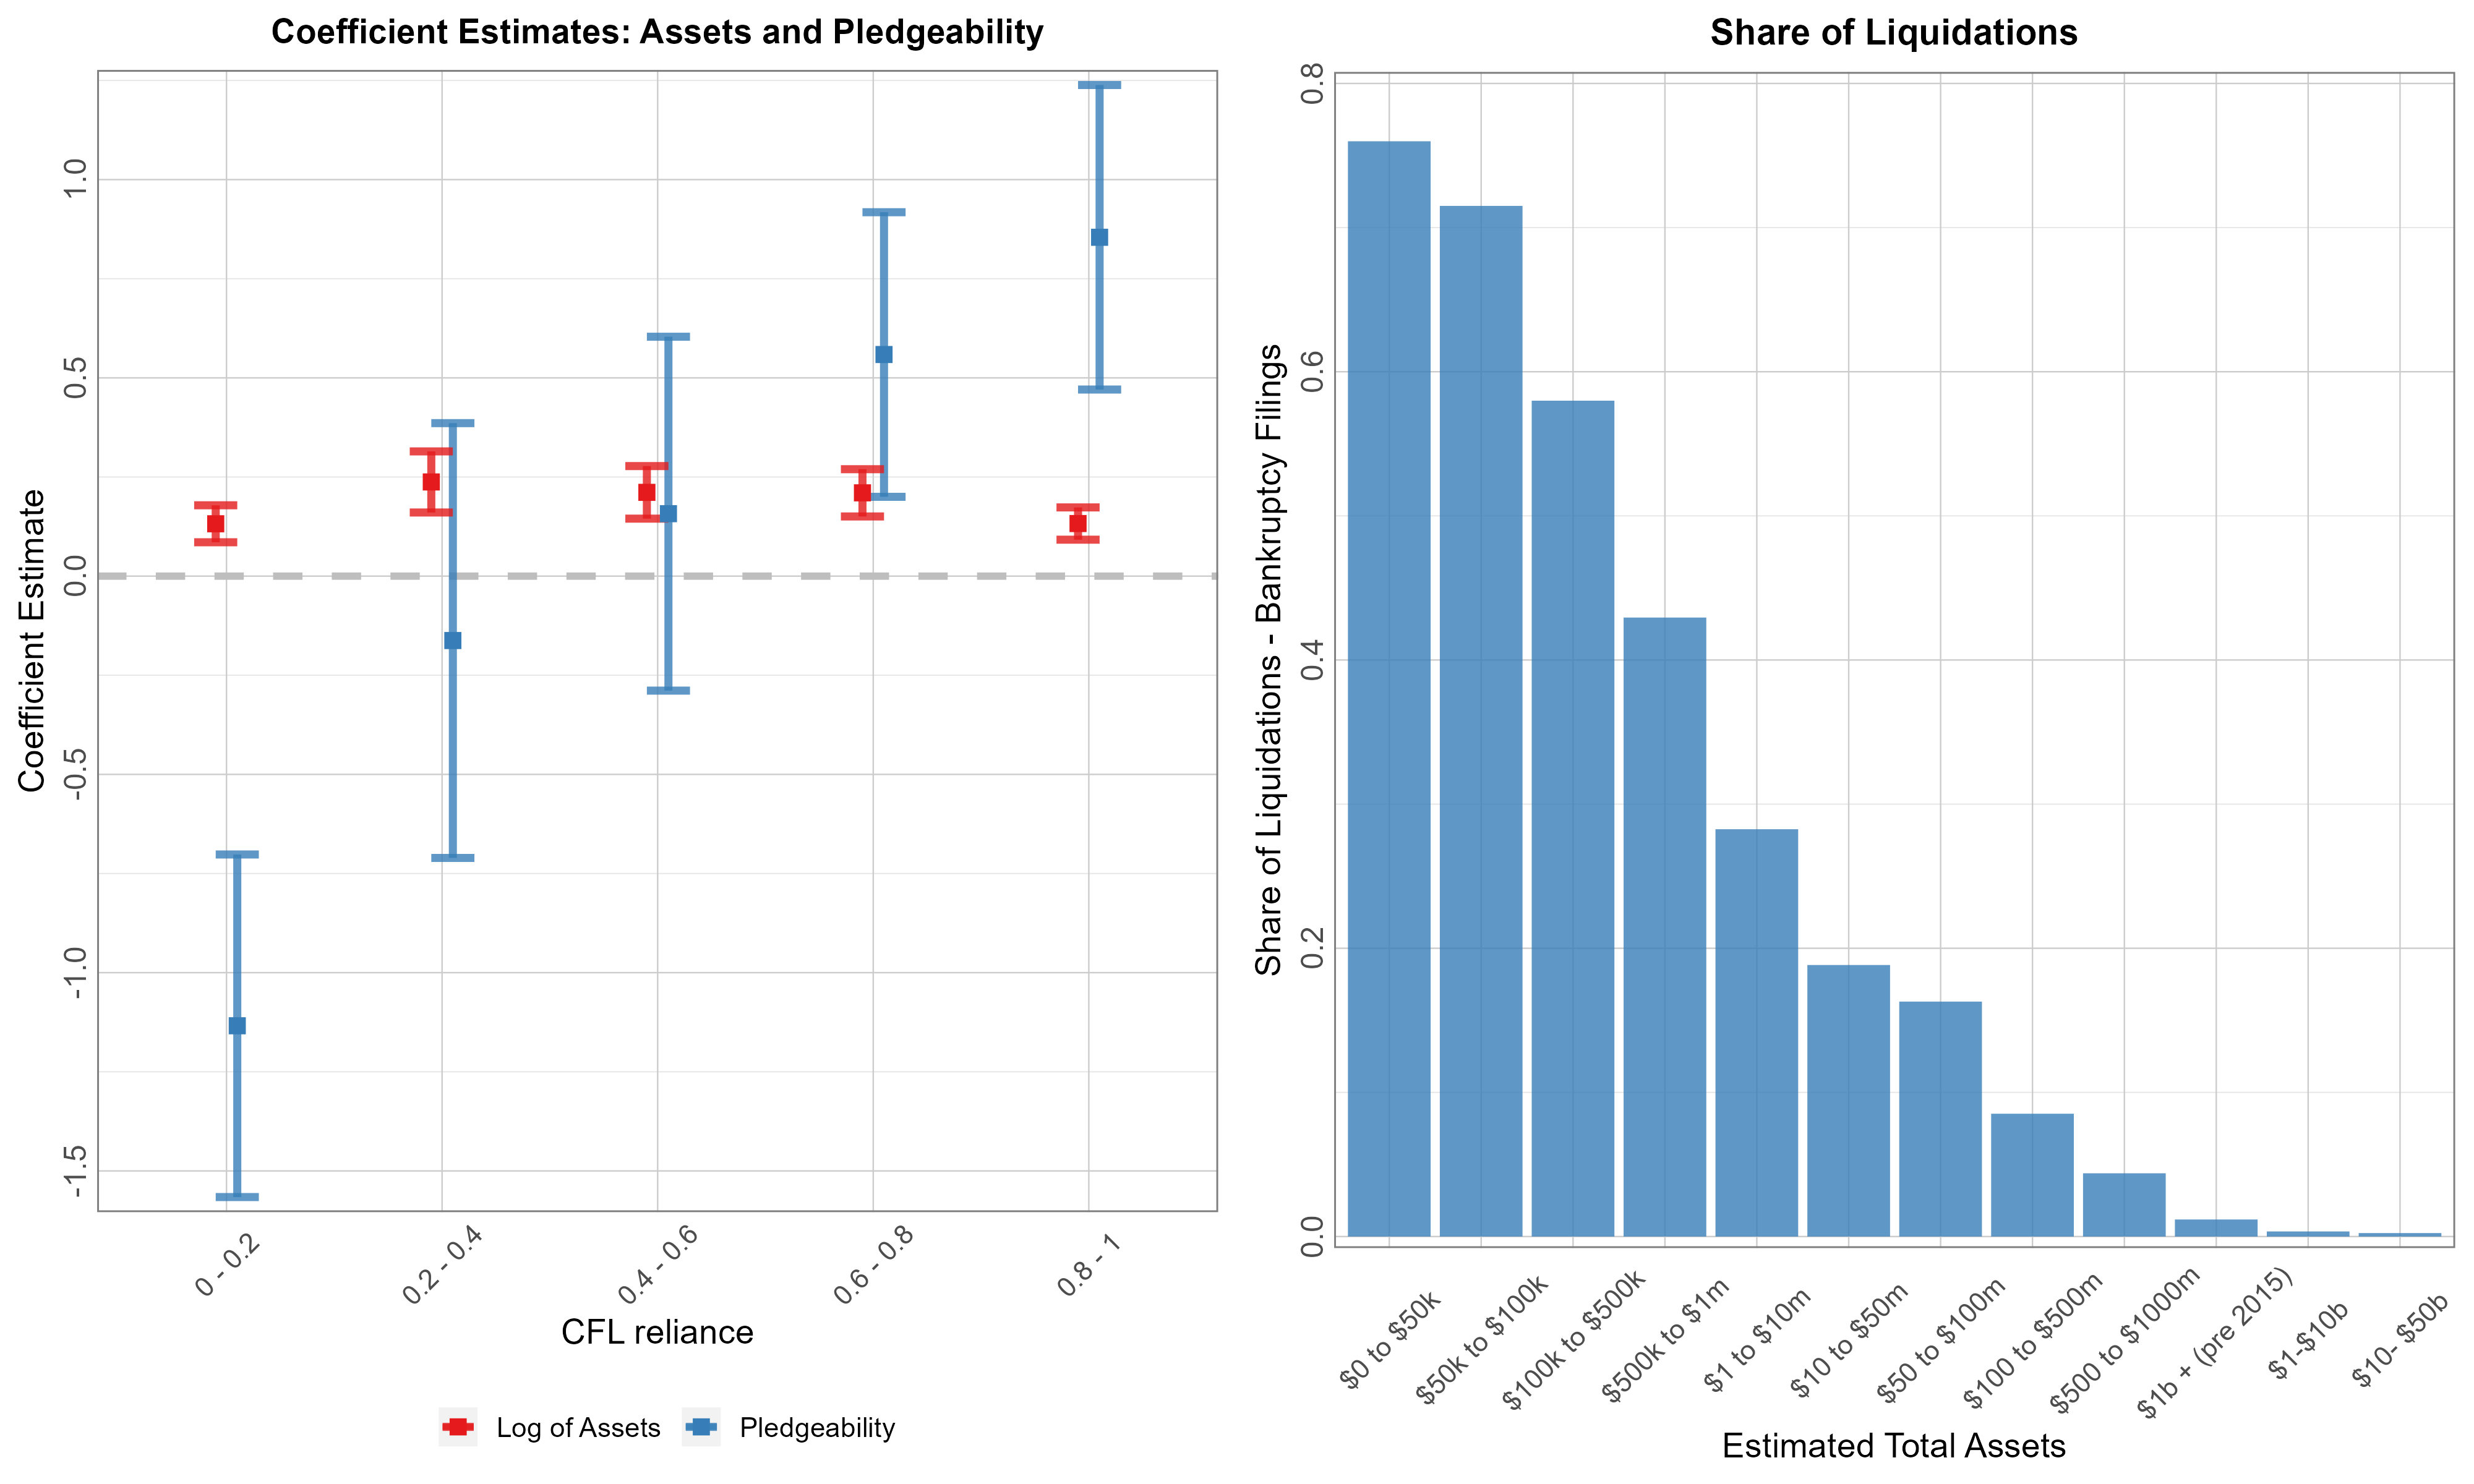
\includegraphics[width=1\textwidth]{C:/Users/szjud/OneDrive/Asztali gép/EBCs/CFL-git/Latex codes/Plots/mixplot.png}
     \footnotesize \justifying Panel A. present coefficient estimates from from the baseline specification for five groups of firms, categorized by their CF-share. The squares represent the coefficient estimates and the error bars show the 95\%  confidence intervals. Panel B. presents the liquidation decision across firm sizes. The bars show the number of bankrupt firms that got liquidated (Chapter 7.) over the total number of bankruptcy filings.
\end{figure}
\newpage 

\noindent To test the robustness of these results, I study these determinants in alternative specifications. Credit spreads have to be calculated manually, as a difference of the interest rate and the T-bill rate at the corresponding maturity. Calculating credit spreads such as this is subject to some uncertainty, therefore I consider the same models with interest rate as the dependent variable. In this case, I add maturity at the time of issueance to the control variables. These results are presented in table ... and ... of the appendix. Moreover, I repeat the debt-level regression on credit spreads without limiting the sample to new issuances - this regression is reported in table ... of the appendix. The qualitative predictions of these empirical models remain virtually unchanged in every alternative specification.

\subsection{Further Determinants of Credit Spreads\label{sec:credit spreads}}
Higher leverage has associated higher credit spreads in every specification, but this effects is somewhat larger for CF-based debt. This is intuitive as both the probability of default and lenders' exposure increases with debt. The logarithm of age is mostly associated with a significant, negative effect on credit spreads. This could reflect the importance of creditor and debtor relations, in decreasing the external finance premium. Somewhat surprisingly, age tends to have a stronger effect on asset-backed debt. The coefficient estimates the logarithm of the number of employees are not consistent across specifications. This variable have a limited economic impact, even when they are statistically significant, which indicates that assets are a sufficient measure of firms size. \vspace{3mm} \\
In each regression considered here, I include period and sector fixed effect - (the full specification is detailed in ... and ... in the appendix). Sector fixed effects have only a modest effect on credit spreads, which is partly due to also considering pledgeability as a separate variable. Moreover, I control for the credit ratings. These have large impact on the borrowing conditions. Consistent with the view that lender perception matters more in the case of CF-based debt, a worse rating is associated with strong increase in external finance premium. In contrast, for asset based debt contracts, credit spreads only react to credit ratings that are associated with high default risk.  \vspace{3mm} \\
Firms often rely on multiple debt contracts simultaneously, holding both cash flow-based and asset-based debt simultaneously. I measure firms' reliance to CF-based lending as the share of CF-based debt to total debt. This measure of `CF-share' is associated with lower spreads for CF-based borrowing and higher spreads for asset-based contracts. This highlights firms' self-selection into asset-based or CF-based borrowing. Firms with cheaper access to CF-based debt or costlier access to asset-based debt (due to some unobserved factors) tend rely more heavily on CF-based financing. \vspace{3mm} \\
Further inspection of CF-share, shows that only a small segment of overall market relies exclusively on one type of debt. That is, 35.7\% of firms use only asset-based debt, and 12.2\% rely solely on cash flow-based financing (CF-share of 0 and 1 respectively). The rest, 52.1\% of firms simultaneously hold both type of debt contracts. Since these are often the largest corporations, they correspond to 87.3\% of the market by the value assets and 90.3\% by the value of borrowing. This further highlights the limitations of classifying firms into two non-intersecting groups of borrowers, subject to asset-based or earnings-based frictions.

\subsection{Limitations}
Empirical analyses of the determinants of credit spreads must contend with certain limitations. First, credit spreads and debt financing strategy are jointly determined, meaning that firms' endogenous reaction to credit conditions, influences the interest rates they eventually face. Therefore, without relying on natural experiments, it often is not possible to identify causal effects. Other potentially important determinants are not observable. In this paper, I argue that one such factors is lenders' expectations that the firm would liquidate under financial distress, but assets specificity (Kermani and Ma, 2020) or the quality of accounting practices and court enforceability (Lian and Ma, 2021) are similarly elusive. The structural model discussed below makes up for some of these limitations. 

\section{Model outline} \label{sec:model}

In this section, I study the determinants of credits spreads in a partial equilibrium model of firm policies. The model describes the effects of leverage, productivity, and total assets on credit spreads. Moreover, it highlights that credits spreads of CF-based debt contracts increase with the probability that the firm would be liquidated under financial distress. This determinant, despite its considerable impact on access to debt finance, has been overlooked by previous structural analyses. Since small firms are frequently liquidated, their access to cash flow-based debt is hindered. The resulting misallocation of capital yields significant productivity losses. \vspace{3mm} \\
To keep the model parsimonious, I do not consider differences in asset pledgeability or asset specificity. This would be a straightforward extension to the model, but incorporating an additional state variable (describing firm-specific asset pledgeability) would make the computational burden unmanageable.\footnote{Öztürk (2023), considers the effects of this determinant of firms optimal debt financing strategy.} Finally, I do not consider effects of firm age on credit conditions. To explore the effects of this determinant, one would have to consider a Bayesian learning mechanism similar to Kochen (2022) as well as information asymmetries between creditors and lenders. This is beyond the scope of this paper. 

\subsection{Firms and production \label{sec:production}}
Heterogeneous firms produce a homogeneous consumption good, using labour, $n$ and capital, $k$. Firms are competitive, and face a decreasing returns to scale production technology:
\begin{equation} \label{eq:prodf}
y = \varepsilon k^{\alpha}n^{\nu}, \ \ \ \ \alpha,\nu \in (0,1),  \ \nu + \alpha \in (0,1)
\end{equation}  
where $\varepsilon$ is the idiosyncratic productivity state. In the interest of keeping the notation simple, I omit firm subscripts. \vspace{3mm} \\
Firms own capital and investments are financed partly by financial wealth and partly by borrowing from a competitive lender. A firm can be described by the predetermined capital stock $k \in \mathbf{K} \subset \mathbf{R^{+}}$, debt\footnote{Firms may also decide to save in which case their debt towards the intermediary is negative.} $b \in \mathbf{B} \subset \mathbf{R}$ and current productivity $\varepsilon \subset \mathbf{R^+}$. Idiosyncratic productivity is a Markov chain on the finite set $\varepsilon \in \mathbf{E} \equiv \{ \varepsilon_1,...,\varepsilon_{N_{\varepsilon}} \}$ such that $ g_{ij} \equiv \Pr(\varepsilon'= \varepsilon_j|\varepsilon = \varepsilon) \geq 0$ and $\sum_{j=1}^{N_{\varepsilon}} g_{ij} = 1$ for each $i$. Moreover, it is stochastically monotone such that for any fixed $x$, $\Pr(\varepsilon' \leq x | \varepsilon = \varepsilon_i)$ is decreasing in $\varepsilon_i$. \vspace{3mm} \\
Production occurs before the realization of exit and entry decisions take effect, and optimal labor demand is independent of current debt. Therefore, every firm with the state vector at the beginning of the period $(k,\varepsilon)$ faces the same static optimization of labour: 
$$ \pi(k,\varepsilon) = \max_{n} \ \  \varepsilon k^{\alpha}n^{\nu} - wn - c$$
where $c$ is a fixed cost of participating in production, $w$ is equilibrium wage and the price of the consumption good is flexible and normalized to $1$. Optimization yields the policy function for labour demand, $n(\varepsilon,k)$ and optimal production $y(\varepsilon,k)$: 
\begin{equation} \label{eq:opt_emp_prod}
n(k,\varepsilon) = \left( \dfrac{ \nu \varepsilon k^\alpha}{w} \right)^{\frac{1}{1-\nu}} \hspace{15mm}
y(k,\varepsilon) = \varepsilon k^{\alpha} \left( \dfrac{\nu \varepsilon k^\alpha}{w} \right)^{\frac{\nu}{1-\nu}}
\end{equation}  
Firm profit function can be reformulated as: 
\begin{equation} \label{eq:profit}
\pi(k,\varepsilon) = y(k,\varepsilon) - wn(k,\varepsilon) - c = (1-\nu) y(k,\varepsilon) - c
\end{equation} 
Active firms own capital and make idiosyncratic investment decisions. Capital accumulation follows: 
\begin{equation} \label{eq:capital}
k' = (1-\delta)k + i
\end{equation} 
where $\delta$ is the depreciation rate and $i$ is investment. Capital adjustment is not subject to microeconomic frictions. Moreover, the lending schedule faced by individual firms depends only on future values of capital and debt, which firms may choose independently from current stocks. Hence, firms' financial position at any given period can be summarized by a cash on hand variable, $x \in \mathbf{X}$: 
\begin{equation} \label{eq:cash on hand}
    x = \pi(k,\varepsilon) + (1-\delta)k - b 
\end{equation}
The cash on hand and current productivity, $(x, \varepsilon)$ describe firms' current state. Hence, it is possible summarize the distribution of firms using the probability measure $\mu$ defined on the Borel algebra $A$, generated by the open subsets of the product spaces $ \mathbf{A} = \mathbf{X} \times \mathbf{E} $.  This reformulation reduces the computational burden the model. 

\subsection{Firm Values and the Default Decision \label{defaults}} 
Production takes places at the beginning of the period. Firms set their labour demand given $(k,\varepsilon)$, profits are realized and capital depreciates. Then, incumbents may decide to exit, default or continue production to the next period. This decision is governed by: 
\begin{equation} \label{eq:default decision}
    V(x,\varepsilon) = \max \{ V_{def}, V_{exit}(x), V_{cont}(x,\varepsilon) \}.
\end{equation}
Default is associated with zero value regardless of the prior state or the eventual default resolution, such that $V_{def} = 0$.\footnote{This assumption reduces the computational complexity of the model on two accounts. It enables combining capital and debt into a single cash on hand variable and allows firms to solve optimal CF-reliance independently from the rest of the optimization. As for its impact on model results, it means that firms do not adjust their debt financing strategy to retain more value after bankruptcy. Omitting this aspect of the optimization likely has modest effects on the model results.} Alternatively, firms may choose to exit without falling back on limited liability, retaining the value of the depreciated capital stock net of debt service. Hence, in an orderly exit, the firm can keep its cash on hand, with $V_{exit} = x$. Figure \ref{chart:DEC} in the appendix summarizes firms' decision on given current cash on hand and continuation value. \vspace{3mm} \\
Firms that decide to continue have access to external finance in the form of one-period debt contracts. For every unit of debt to be repaid in the next period, they receive $q$ units of output that may be allocated towards investment or distributed as dividends. It is possible to borrow against physical assets or future cash flows. These debt contracts differ in their in-default payoffs. Asset-based contracts yield better payoffs under liquidation, while CF-based contracts extract more value under reorganization - I discuss these in detail in the following section. In every other respect, the two loan-types are the same. Total debt can be described as $b = b^C+b^A$, and analogously to the empirical analysis, I define CFL reliance as: 
\begin{equation}
    \tau = b^C/(b^C+b^A).
\end{equation}
Continuing firms choose future capital stock, $k'$, total future debt, $b'$ and debt financing strategy $\tau'$ to maximize the discounted sum of dividends, $d$ 
\begin{equation} \label{eq:dividends}
d = x - k' +  q(k',b',\varepsilon, \tau')b'
\end{equation} 
the value of continuation is described by:
\begin{equation} \label{eq:V_cont}
    V_{cont}(x,\varepsilon) = \max_{k',b', \tau'} \left(x - k' +  q(k',b',\varepsilon, \tau')b' + \beta \E_{\varepsilon'|\varepsilon} V(x',\varepsilon') \right)
\end{equation}
subject to: 
\begin{equation} \label{eq:budget}
x' = \pi(k',\varepsilon')+(1-\delta)k'-b' \hspace{5mm} \text{and} \hspace{5mm} d \geq 0.
\end{equation}
In order to simplify notation, I summarize the collection of decision variables introduced above as: $a = (k, b, \tau) $. In the next section, I discuss how the inverse gross interest rate $q(a',\varepsilon)$ depends on these decision variables and the current productivity.

\subsection{Financial Intermediation}  \label{sec: Financial Intermediation}
\subsubsection{The lender's problem}    \label{sec: The lender's problem}
The opportunity cost of lending to corporations is determined by the risk-free bond yields $q_0$ - in partial equilibrium, this is set to be equal $\beta$. Since corporate lending is risky, the competitive lender must charge a premium to break even. When setting $q(a',\varepsilon)$ the lender must consider the expected payoff under 3 distinct scenarios: \textit{a)} orderly repayment; \textit{b)} the firm defaults and is liquidated \textit{c)} the firm defaults and is reorganized.\footnote{Note that the lender cannot retrieve more than the initial value of the debt, which is made sure by the minimum function in \ref{eq:q}.}  It follows from the zero-profit condition that the debt schedule offered to firms is, 
\begin{equation} \label{eq:q}
    \begin{split}
        & q(a', \varepsilon)b' =  \beta \left[ (1-P_D(a', \varepsilon))b' + \right. \\
        & \quad P_D(a', \varepsilon) \min \{b, \ \gamma(a', \varepsilon) \Pi_{liq}(a') +  \left. (1-\gamma(a', \varepsilon)) E_{\varepsilon'|\varepsilon} \Pi_{reorg}(a', \varepsilon) \} \right] 
    \end{split}
 \end{equation}
where 
\begin{itemize}\setlength\itemsep{0em} 
    \item $P_D(a', \varepsilon)$ is the endogenous probability of default,
    \item $\Pi_{liq}(a')$ is the expected payoff if the firms undergoes liquidation,
    \item $\Pi_{reorg}(a', \varepsilon)$ is the expected payoff if the firms undergoes reorganization,
    \item $\gamma(a', \varepsilon)$ is the probability of liquidation under financial distress. 
\end{itemize} 
In the following, I discuss the default resolution process and the lender's payoffs given the debt contract that is in place at the time of bankruptcy. The goal of this discussion is to explore how the four values introduced above are by influenced the current state and firms' decisions, which further leads to the complete description of the debt schedule $q(a', \varepsilon)$.
 
\subsubsection{Default Resolution and Lenders' Payoffs}   \label{sec:Default Resolution}
This section provides a stylized description of the default resolution process. In practice, this often entails negotiations between the borrower and multiple creditors with potentially conflicting interests, under the supervision of courts. Moreover, the negotiating parties' bargaining power may depend on the specific terms outlined in the contract. I do not attempt to capture all this complexity in the model. Instead, my focus is on providing an accurate description of lenders' expected in-default pay-offs depending on the debt contract that is in place. These are the focus of my analysis, as they determine the trade-offs between lending against assets or cash flows, as well as the interest rates firms eventually face. \vspace{3mm} \\
Bankruptcy may be resolved either through liquidation or reorganization. When a bankrupt firms is liquidated, it exits and the undepreciated capital stock is resold at a discount. The total value retained under liquidation is $\phi_l(1-\delta)k$, where $\phi_l \in (0,1)$ indicates that corporate assets are often highly specialized and illiquid, which limits the resale value. Under reorganization, the household must pay a share of the continuation value to the lender as a lump-sum, in order to allow the firm to carry on to the next period. The maximum value the lender may recover under reorganization is $\phi_c V_{cont}(x,\varepsilon)$, where $\phi_c \in (0,1)$ indicates that the lender cannot capture the entire continuation value. Naturally, this not an accurate description of the reorganization process, but it captures that in this case lenders' payoffs depend on the continuation value of the firm.\footnote{In practice, the means of extracting the continuation value depends on debt the contract in place. When debt is secured against the entire corporate entity, the lender may gain direct access to borrower's cash flows. When the debt is unsecured, higher continuation value of the firm allows the lender to negotiate better terms during reorganization - see Corbae and D'Erasmo (2021).}  \vspace{3mm} \\ 
The values above represent the total value that could be extracted from bankruptcy. However, the actual amount recovered by the lender also depends on the debt contract adopted prior to bankruptcy. Next, I discuss how much lenders expect to retrieve from these values under different debt contracts. \vspace{3mm} \\ 
Take asset based debt first. The main advantage of these debt contracts is that they provide a quick and cost-effective way to recover in-default payments by liquidating the borrowers' assets. Hence, in case of liquidation the lender can extract the full liquidation value. Similarly, when the borrower undergoes reorganization, secured lenders are protected by the `best interest of creditor' test.\footnote{This is a common theme in bankruptcy codes. The EU Directive refers this as ‘best-interest-of-creditors’ test in OJ L 172/27, art. 49; whereas the US bankruptcy code establishes this principle in 11 U.S. Code § 1129.} This states that creditors cannot be worse off under the reorganization plan than they would be under of liquidation. Therefore, I assume that after asset-backed debt contracts, the lender expects to extract the liquidation value $\phi_l(1-\delta)k$, irrespective of the bankruptcy resolution. \vspace{3mm} \\
In contrast, when the debt contract is backed by future cash flows, the lender expects in-default payments mainly reorganization. In this case, the lender receives $\phi_c V_{cont}(x,\varepsilon)$ from the household after cash flow-based debt. This payoff might be greater than the firm's liquidation value, allowing the lender to offer more lenient credit terms. On the other hand, CF-based contracts are often unsecured, limiting the lender's ability to extract in-default payments from the liquidation of the borrowers' assets. Hence, if liquidation occurs the lender can only retrieve a fraction $\kappa \in (0,1)$ of the total liquidation value of $\phi_l(1-\delta)k$.  \vspace{3mm} \\
Table \ref{tab:lender payoffs} presents the lender's payoffs for each debt contract and default resolution pair. This summarizes the central trade-off in the model. When debt is asset based the lender may reliably expect to retrieve the liquidation value of the firm, irrespective of the default resolution. When debt is CF-based the lender expects to retrieve a share of the continuation value under reorganization, but risks of losing out under liquidation.

\begin{table}[h!]
    \centering
    \begin{tabular}{l|cc}
        & Liquidation  & Reorganization \\  
       \midrule
      Asset based contract & $ \phi_l (1-\delta) k$  &  $ \phi_l (1-\delta) k$ \\
      CF based contract & $ \kappa \phi_l (1-\delta) k $ & $ \phi_c V(x,\varepsilon)$ \\ 
     \bottomrule
     \end{tabular}
    \caption{\small The lender's payoffs under each default resolution, debt contract pair gross of fixed costs.} 
    \label{tab:lender payoffs}
\end{table}
\noindent  Finally, similarly to Corbae and D'Erasmo (2021), I assume that both liquidation and reorganization incur fixed costs. The fixed cost of liquidation $\zeta_l$ is a calibration parameter that adjusts the overall accessibility of debt finance. It is set to a relatively low value and is entirely paid by the lender. The fixed cost of reorganization $\zeta_c$ is paid entirely by the household and is calibrated to be high, allowing only the largest and most productive firms to reorganize. The fixed cost of reorganization is crucial for replicating the decreasing liquidation probability in the function of firm size - these fixed costs are discussed in more detail in section \ref{sec:fixed costs} of the appendix.\footnote{The alloaction of these costs may seem somewhat arbitrary. However, note that the incidence of these costs has only a minimal effect credit market frictions. Lenders' expenses directly raise the external finance premium, whereas borrowers' costs limit access to external finance indirectly.}  \vspace{3mm} \\
It is now possible to outline the lender's expected payoff under liquidation and reorganization. As discussed above, the lender's payoff is determined not only by the firm's value but also by the debt financing strategy adopted before the bankruptcy occurs. In the model this is summarized by the CF-reliance, denoted by $\tau$. First, consider the value retrieved after liquidation. The total liquidation value of the firm is: $\phi_l (1-\delta) k$. However, the lender can only retrieve this value for the debt that is backed by a physical assets, which is $1-\tau$ share of the total debt. After the remaining $\tau$ share, the lender can seize $\kappa$ only a fraction of original liquidation value - see bottom-left of table \ref{tab:lender payoffs}. Taking stock, the net payoff that the lender receives from liquidation after paying the fixed costs of reselling assets is:  
\begin{equation} \label{eq:P_liq} 
   \Pi_{liq}(a) = \max \{0, \ (1-\tau) \phi_l (1-\delta) k +\tau \kappa \phi_l  (1-\delta) k - \zeta_l \}. 
\end{equation}
In contrast, CF-backed debt contracts allow lenders to extract the continuation value of the firm. Moreover, in accordance with the `best interest of creditors test', the lender expects to retrieve a payment that is equal to the liquidation value of the collateral after its asset-based debt - see top-right of table \ref{tab:lender payoffs}. Taking stock, when the borrower undergoes reorganization, the lender receives:
\begin{equation}  \label{eq:P_reorg}
   \Pi_{reorg}(a,\tau) = (1-\tau) \phi_l (1-\delta) k +\tau \phi_c V (x, \varepsilon).
\end{equation}
The probability of default set by the default decision described in equation \ref{eq:default decision}. Let $\chi_d(x,\varepsilon)$ be equal to one for all productivity and cash on hand pair that is associated with default. It follows from equation \ref{eq:cash on hand}, that the future cash on hand is the product of the current decisions on capital and debt, such that it is possible to rewrite the future value of this indicator as $\chi_d(a',\varepsilon')$. Hence the probability of default can be summarized in the function of firm decisions and current productivity as follows
\begin{equation} \label{eq:default probability}
    P_D(a',\varepsilon) = \E_{\varepsilon'|\varepsilon}[\chi_d(a',\varepsilon')].
\end{equation}
Finally, to define the probability of liquidation under financial distress, one has to consider the values redistributed to the household after bankruptcy. After liquidation, the lump sum transfer that is redistributed for the household is the total liquidation value net of the lender's payoffs, which amounts to $\phi_l(1-\delta)k - \Pi_{liq}(a)$. Under reorganization the household keeps the firm operational which is associated with value $V(a,\varepsilon)$,\footnote{Here firm value is rewritten with the current decisions on capital and debt, analogously to equation \ref{eq:default probability}.}  but it has to pay a total of $\Pi_{reorg}(a', \varepsilon)$ to the lender as well as the fixed cost of reorganization $\zeta_c$. The household chooses the option that leaves her with the highest value after paying the lender. Therefore, the ex-ante probability of liquidation can be described as
\begin{equation} \label{eq:liquidation probability}
    \gamma(a',\varepsilon) = \E_{\varepsilon'|\varepsilon}[\mathds{1}(\phi_l(1-\delta)k' - \Pi_{liq}(a')  \  \geq \ V(a',\varepsilon') - \Pi_{reorg}(a', \varepsilon') - \zeta_c)].
\end{equation}
The assumption that lenders' payoffs are not considered at the liquidation decision reflects the fact that individual lenders often have a limited influence over the default resolution - see in section \ref{sec:key principles} of the appendix.\footnote{Alternatively, it could be assumed households also into account the lender's payoffs. In this case the liquidation decision would be described by: $\phi_A (1-\delta) k - \zeta_l  \  \geq \ \phi_C V_2(x,\varepsilon)- \zeta_c$. This is also a plausible assumption, and I am still considering it as it has several advantages. The problem is that it cannot reproduce CFL reliance between zero and one.} \vspace{3mm} \\
This completes the discussion of the four values necessary to describe the interest rate schedule $q(a', \varepsilon)$. The next section discusses the optimal debt financing strategy of firms, given these values. 

\subsubsection{Optimal debt financing strategy}
As mentioned above, firms associate zero value with bankruptcy irrespective of the default resolution. This assumption simplifies the solution of the model as it implies that the debt financing strategy only affects firm values through the current external finance premium. Moreover, since firm value is monotonously increasing in $q(k',b',\varepsilon, \tau')$, for any $(k',b',\varepsilon)$ the optimal debt financing strategy coincides with choosing the $\tau'$ that maximizes the inverse gross interest rate. Substituting equation \ref{eq:P_liq} and \ref{eq:P_reorg} into \ref{eq:q} and using that $q_0 = \beta$, it is possible to express the optimal CFL reliance as follows:
\begin{equation} \label{eq:opt_tau}
    \begin{split}
        & \tau^*(k',b',\varepsilon) = \argmax_{\tau'} \ \  \frac{\beta}{b'} \Big{[} (1-P_D(a', \varepsilon))b' \ +  \\
        & \quad  P_D(a', \varepsilon) \min \big{\{} b', \ \gamma(a',\varepsilon) \max \{0, \ (1-\tau) \phi_l (1-\delta) k +\tau \kappa \phi_l  (1-\delta) k - \zeta_l \} +  \\
        & \quad (1-\gamma(a',\varepsilon)) \left(  (1-\tau) \phi_l (1-\delta) k +\tau \phi_c V (x, \varepsilon) \right) \big{\}} \Big{]} 
    \end{split}
 \end{equation}
Note that firms may avoid paying a risk premium by adopting a debt financing strategy that allows the lender to recover the entire debt value in every future state, or accumulating enough assets such that the probability of default becomes zero. For these firms, the debt financing strategy does not affect the interest rate they are charged. To associate a debt financing strategy to these firms, I assume they borrow against assets if their liquidation value is higher and against cash flows if their reorganization value is higher. \vspace{3mm} \\
Using the expression for the optimal CFL reliance, firms dynamic optimization can be reformulated as, 
    \begin{equation} 
        V_{cont}(x,\varepsilon) = \max_{k',b'} \left(x - k' +  q(k',b',\varepsilon)b' + \beta \E_{\varepsilon'|\varepsilon} V(x',\varepsilon') \right)
    \end{equation}
    subject to: 
    \begin{equation} \label{eq:cont_1}
    x' = \pi(k',\varepsilon')+(1-\delta)k'-b'; \hspace{10mm} d \geq 0;  \hspace{10mm} \tau' = \tau^*(k',b',\varepsilon)
    \end{equation}

\subsection{Firm dynamics}
In the previous section, I defined the indicator function: $\chi_d = 1$ if the firm decides to default on its debt. Moreover, I define $\chi_l = 1$ if the firm is liquidated under financial distress and $\chi_{ex} = 1$ if the firm exits voluntarily, after repaying its debt. The combination of these indicator functions describe the possible resolutions the debt contract, summarized by \ref{table:indic}.  \\
\begin{table}[h!]
    \centering
    \begin{tabular}{|c|c|c|c|} 
    \hline
    Case &$\chi_d $ - default & $\chi_l$, \ $\chi_{ex}$ - exit &  Outcome  \\ \hline
    1. & $\chi_d = 0 $ &  $\chi_{ex} = 0$  & Repays debt, Continues \\
    2. & $\chi_d = 0$ &  $\chi_{ex} = 1 $  & Repays debt, Exits   \\
    3. & $\chi_d = 1$ &  $\chi_l = 0$  & Defaults, Continues  \\
    4. & $\chi_d = 1$ &  $\chi_l = 1$ & Defaults, Exits \\ 
    \hline
    \end{tabular}
    \caption{Possible debt contract resolutions in the model}
    \label{table:indic}
\end{table}

\noindent At each period, firm exits are balanced by a mass $M$ of potential entrants. These are endowed with zero starting cash on hand (to reflect the fact that startups are typically asset-poor) and a starting productivity that is drawn from stationary distribution of the Markov chain defining idiosyncratic productivity. In the following, this distribution is denoted by $\Phi(\varepsilon)$. Entrants do not produce in the first period, and they have the option to exit immediately if their continuation value is smaller than zero. Thus, potential entrants essentially face the same optimization as incumbents - the only difference is that their cash on hand is always zero.\vspace{3mm} \\
Let $\mu_0$ be the measure of the mass of firms at the beginning of the period. Using the indicator variables defined above, the measure of firms at the end of the period can be defined as: $\mu = \mu_0( 1 - \chi_d\chi_l - (1-\chi_d)\chi_{ex} )  + \chi_{ex}M d \Phi(\varepsilon) $. The evolution of firm distribution then satisfies:
\begin{equation} \label{eq_firmdim} 
    \mu_{0}'(A) = \int \mathbf{I}_{(x', \varepsilon') \in A} g(\varepsilon'|\varepsilon) \ d \mu (x,\varepsilon)
\end{equation}
for all Borel sets $A \subset  \mathbf{X} \times \mathbf{E} $ and where $g(\varepsilon'|\varepsilon)$ is the transition probability matrix idiosyncratic productivity. I summarize the dynamics of firm distribution at the end of the period by the mapping $ \mu' =\Gamma(\mu)$.

\subsection{Stationary equilibrium}\label{sec:eq}
In the partial equilibrium, households inelastically provide a labour supply of $N^S$ such that the equilibrium wage is determined entirely by the aggregate labour demand of firms. Moreover, household invest into risk free bonds $B$ such that risk free interest rate $q_0$ is equal to the discount parameter $\beta$ and consume $C$ in each period. The stationary competitive equilibrium can be described by the set of functions
$$(\mu_0, \mu, w, V, V_{cont}, V_{ex}, \chi_l, \chi_d, \chi_{ex}, l,q,k,b,d)$$
such that: 
\begin{enumerate}[(i)]
\item Firms solve value maximization. $V$ solves \ref{eq:default decision} and $V_{cont}$ solves \ref{eq:profit}, \ref{eq:V_cont} and \ref{eq:budget}; and the associated policy functions are $l$, for exiting and defaulting firms and $(l,k,b,d,q)$ for continuing firms.
\item Labour market clears: 
$$ N^s = \int n  \ d \mu_0 (x,\varepsilon)  $$
\item Financial market clears:
 $$ B = \int b \ d \mu_0 (x,\varepsilon) $$
\item Goods market clear: 
$$ C + I = \int y \ d \mu_0 (x,\varepsilon)$$
where aggregate investment is the sum of investment carried out by continuing firms and startups minus the capital freed up due to liquidations and voluntary exits:
\begin{multline*} 
    I = \int   k' -(1-\delta)k \ d \mu (x,\varepsilon) - \int \chi_d \chi_l \phi_l(1-\delta)k \ d \mu_0 (x,\varepsilon) \  - \\
    \int (1-\chi_d)\chi_{ex} (1-\delta) k \ d \mu_0 (x,\varepsilon)  + M \int (1-\chi_{ex}) k' \ d \Phi(\varepsilon) 
\end{multline*}
\item The distribution measure of active firms is stationary, $\Gamma(\mu) = \mu$ and prices $(w,q)$ are constant over time.
\end{enumerate}

\newpage

\section{Calibration}

The model is calibrated at a yearly frequency. Parameter values that are calibrated externally are taken from comparable structural models such. Moreover, recovery rates $\phi_l$ and $\phi_c$ are set following the empirical estimates of Kermani and Ma (2020). These are summarized in table \ref{tab:external calib}: 

\begin{table}[h!]
    \centering
    \begin{tabular}{c|c|c|c}
    \toprule
    \textbf{Parameter} & \textbf{Name} & \textbf{Value} & \textbf{Source} \\
    \midrule
    $\alpha$ & Capital Share & 0.33*DRS & Jo and Senga (2019) \\
    $\nu$ & Labor Share & 0.67*DRS & Jo and Senga (2019) \\
    $\beta$ & Discount Rate & 0.96 & Convention \\
    $\delta$ & Depreciation & 0.06 & Khan and Thomas (2013) \\
    $\rho$ & Shock Persistence & 0.969 & Di Nola et al. (2023) \\
    $\sigma_{\varepsilon}$ & Shock SD & 0.146 & Di Nola et al. (2023)  \\
    $\varepsilon_0$ & Average Productivity & 1 & Di Nola et al. (2023)  \\
    $\phi_l$ & Resale value of assets & 0.4 & Kermani and Ma (2020) \\ 
    $\phi_c$ & Recovery in liquidation & 0.8 & Kermani and Ma (2020) \\    
    \bottomrule
    \end{tabular}
    \caption{Externally calibrated parameters parameter values and sources}
    \label{tab:external calib}
\end{table}
\noindent Idiosyncratic firm productivity follows the AR(1) process,
$$ \ln(\varepsilon_{t+1}) = (1-\rho) \ln(\varepsilon_0) + \rho \ln(\varepsilon_t) + \sigma \zeta_\varepsilon $$
\begin{itemize}\setlength\itemsep{0em} \small
    \item $\rho$ is the persistence of productivity the shock
    \item ln($\varepsilon_0$) is the average productivity
    \item $\sigma$ is the standard deviation of shocks
\end{itemize} \normalsize
With probability $P_{exo} = 0.03$ firms may receive a negative productivity shock such that they must exit or liquidate depending in the cash on hand available to them. Since this shock always leads to firm exit, I do not define how productivity after it. This assumption ensures that most firm do not grow out of financial constraints in their lifespan. I discretize the log-process via Tauchen's method. \vspace{3mm} \\ 
Bankruptcy codes often contain special provisions to facilitate reorganization of SMEs, based on the recognition that reorganization costs are often prohibitive for small corporations - see section \ref{sec:key principles} of the appendix. To reflect this fact in the baseline calibration, I assume that the bottom quintile of firms pay a reduced fixed cost $\zeta_{cs}$. The rest of the firms pay the full cost of reorganization $\zeta_{cl}$. These parameters are calibrated internally to match the average firm-level reliance on CF-based debt and the share of CF-debt to total debt in the economy. These and other internally calibrated parameters are summarized in \ref{tab:internal calib} while target values are summarized in \ref{tab:targets}.

\begin{table}[h!]
    \centering
    \begin{tabular}{c|c|c}
    \toprule
    \textbf{Parameter} & \textbf{Name} & \textbf{Value} \\
    \midrule
    $P_{exo}$ & Negative Productivity Shock & 0.03 \\
    $c$ & Participation Cost & 28 \\
   $ DRS$ & Decreasing Returns to Scale & 0.75 \\
    $\zeta_{cl}$ & Fixed Cost of Reorganization - Large firms & 8500 \\
    $\zeta_{cs}$ & Fixed Cost of Reorganization - Small firms & 2500 \\
    $\zeta_l$ & Fixed Cost of Liquidation & 200 \\
    $\kappa$ & Discount for CF-based Debt after Liquidation & 0.5 \\
    \bottomrule
    \end{tabular}
    \caption{Parameter Values}
    \label{tab:internal calib}
\end{table}

\begin{table}[h!]
    \centering
    \begin{tabular}{c|c|c|c}
    \toprule
    \textbf{SS value} & \textbf{Target value} & \textbf{Model value} & \textbf{Related params.} \\ 
    \midrule
    Debt to Collateral & 0.51 & 0.51 & $\zeta_l$, $P_{exo}$\\
    Average interest rate & 4.9 & 4.3 &  $\zeta_l$, $P_{exo}$  \\
    Share of CF debt & 0.767 & 0.767 &  $\zeta_{cl}$ \\
    Average CF-reliance & 0.45 & 0.465 &  $\zeta_{cs}$ \\
    Liquidation prob. & 0.50 & 0.41 & $\zeta_{cl}$, $\zeta_{cs}$ \\
    Exit share & 0.09 & 0.11 & $c$, $DRS$ \\
        \bottomrule
    \end{tabular}
    \caption{Target and model values}
    \label{tab:targets}
\end{table}

\newpage

\section{Results}
 
In the following, I present preliminary results of the structural analysis. First, I consider steady state values under alternative model calibrations, different only in the fixed cost of reorganization $\zeta_c$. I consider four distinct cases. The baseline case where $\zeta_{cs} = 3000$ for small corporations (bottom quintile by assets) and $\zeta_{cl} = 8500$ for large enterprises. This calibration of the model fits the best to the targeted moments in the data. The cost of entry set to equate the equilibrium wage to one. \vspace{3mm} \\
Second, I consider a calibration where the fixed costs of reorganization is prohibitive such that firms are always liquidated. In this case, CF-based contracts always perform worse, meaning that no firms chooses to borrow against future cash flows. Compared to the baseline case, debt to capital falls by 14 percentage point. This implies startups take longer to reach their efficient sizes, which decreases the value of entry. As a result, the mass of firms and the equilibrium wage declines. Average productivity, which is proportional to the wage, declines as well, by 1.7\%. This decline can be interpreted as the productivity loss that would be suffered if CF-based contracts did not exist. \vspace{3mm} \\
Next, consider the scenario where the fixed costs of reorganization are reduced to match the fixed cost of liquidation. This would improve credit conditions by a large margin. Total debt-to-assets ratio would increase nearly threefold, although this would come with significantly higher funding cost. Such a change would imply a productivity improvement of 7.2\%. This scenario is arguably not very realistic, but it indicates that reducing the fixed costs of reorganization has a considerable potential to increase productivity. Finally, I consider a perfect credit economy, where firms had access to equity finance at a zero cost. In the absence of credit market frictions aggregate productivity increases by 15.05\%.

\newpage

\begin{table}[h!]
    \centering
    \begin{tabular}{lcccc}
    & \textbf{Prohibitive} & \textbf{Baseline} & \textbf{Best case} & \textbf{Perfect Credit} \\
    \toprule
    \multicolumn{1}{c}{$\zeta_{cl}$ and $\zeta_{cs}$} & $\infty$ & 8500, 3000 & 200, 200 & - \\
    \multicolumn{1}{c}{$\zeta_l$} & 200 & 200 & 200 & \ - \vspace{3mm} \\
    \multicolumn{5}{l}{\textbf{Aggregates}} \\ \hline
    Wage & 0.982 & 1 & 1.072 & 1.156 \\
    Y to L & 1.966 & 2 & 2.144 & 2.311 \\
    Total mass & 3.740 & 3.852 & 6.846 & 10.781 \\
    Exit/Entry mass & 0.379 & 0.431 & 1.150 & 0.654 \\
    Exit share & 0.101 & 0.112 & 0.168 & 0.061 \\
    SME share & 0.705 & 0.662 & 0.759 & 0.784 \\
    CF to total debt & 0 & 0.767 & 0.777 &  \ 0.975 \vspace{3mm} \\
    \multicolumn{5}{l}{\textbf{Firm-level averages}} \\ \hline
    Productivity & 1.974 & 2 & 2.144 & 2.311 \\
    Debt to capital & 0.378 & 0.512 & 1.417 & 0.003 \\
    Interest rate & 6.3\% & 4.3\% & 8.2\% & 7.6\% \\
    Liquidation prob. & 1 & 0.412 & 0.331 & 0 \\
    CF reliance & 0 & 0.465 & 0.514 & 0.205 \\
    \bottomrule
    \end{tabular}
    \caption{Comparison of Economic Scenarios}
    \label{tab:SSvalues}
\end{table}

\noindent Next, I study simulations of firms' lifecycle. In this exercise, I consider high productivity entrants and study their evolution over their lifecycle - while also allowing them to be affected by idiosyncratic productivity shocks. For each simulation, I study the first 15 time periods into the future. To make sure that results are not affected by idiosyncratic shocks, I take the average of 100000 simulations. Figure \ref{chart:dynsim}, summarizes these results. The solid blue line represents the prohibitive case and the dashed orange line is the baseline case. Firms behave similarly under both calibrations, accumulating comparable amounts of cash on hand, capital, and debt. However, their financing costs differ significantly between the cases. When firms have access to cash flow-based debt, they pay much lower interest rates (with $q$ closer to one). This enables them to pay more dividends and achieve higher values early in their lifecycle. \vspace{3mm} \\
After five periods, there are no large differences between the baseline and the prohibitive case, which suggest that firms escape financial frictions induced by the lack of pledgeability assets relatively quickly. By this point, firms have accumulated sufficient wealth to fund themselves through asset-based contracts, without a raising their funding costs. The secular decline in most values is attributable to the mean reversion of the productivity process, since i this exercise I consider relatively productive new entrants who, on average, converge to the expected value of the productivity process.

\begin{figure}[H]  % [h] indicates placing the image here
    \centering
    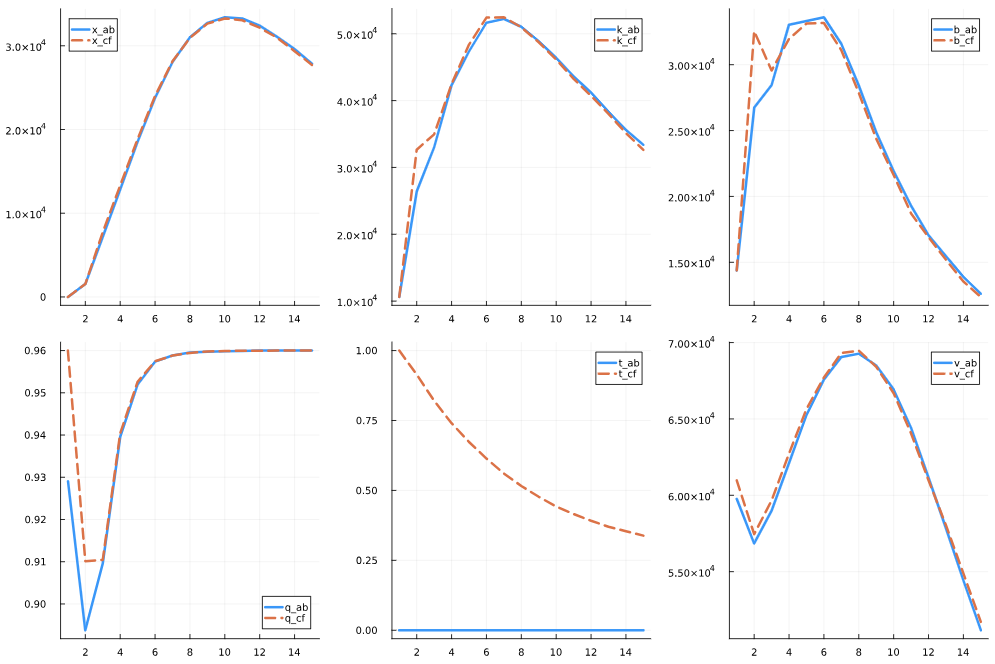
\includegraphics[width=1\textwidth]{C:/Users/szjud/OneDrive/Asztali gép/EBCs/CFL-git/Latex codes/Plots/dynsim.png}
    \caption{Firm lifecycle simulations} \label{chart:dynsim}
\end{figure}

\noindent Figure \ref{chart:DnQ} present a similar piece of evidence. It shows that average optimal policies across firms sizes. On the left panel, I take the 10-base logarithm of average debt. Similarly to the previous exercise, this result indicates that while optimal values of debt do not change for either calibrations the external finance premium is much larger when firms have no access to CF-based debt. 

\begin{figure}[H]  % [h] indicates placing the image here
    \centering
    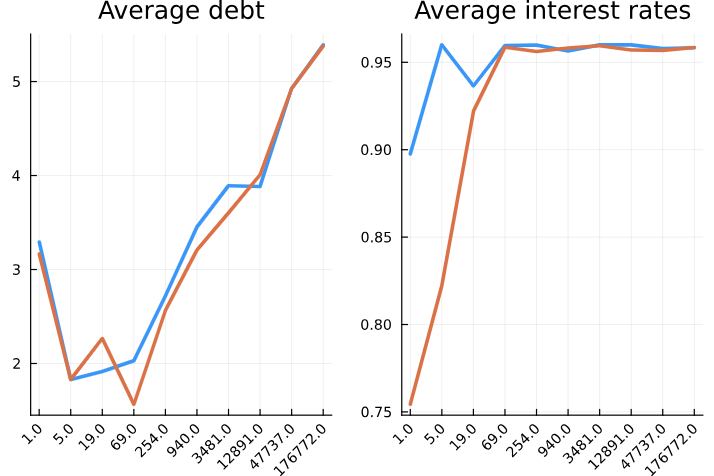
\includegraphics[width=0.9\textwidth]{C:/Users/szjud/OneDrive/Asztali gép/EBCs/CFL-git/Latex codes/Plots/DnQ.png}
    \caption{The log of debt and the inverse gross interest rate across firm sizes} \label{chart:DnQ}
\end{figure}

\noindent Gonzalez and Sy (2024) documents on a comprehensive dataset of Spanish firms that the average reliance on CF-based debt is U-shaped across firms sizes. Interestingly, the US firms covered in Compustat display a similar behavior.  Moreover, as shown in figure \ref{chart:Ushape}, the structural setup proposed here replicates this pattern (even without specifically targeting this result). However, the explanation proposed by Gonzalez and Sy (2024) is fundamentally different to what is suggested by my model. Their explanation rest on the following four assumptions: \textit{1)} firms face a variable cost of pledging collateral; \textit{2)} asset-backed loans have lower interest rates; \textit{3)} there are microeconomic cost of capital adjustment and \textit{4)} the pledgeability of earnings is such that earings-based constraints are less restrictive for small firms. In their model, assumption \textit{1-3} are necessary to match the right hand side of the U-shape and assumption \textit{4} matches the left hand side. \vspace{3mm} \\
In contrast, my model suggests that the optimal reliance on cash flow-based debt is determined by two factors: the relative value of continuation versus pledgeable assets and the probability of liquidation under financial distress. Firms on the left-hand side of the U-shape, typically productive entrants, with scarce pledgeable assets but high continuation values. This makes high reliance to on CF-based debt advantageous to them. On the right-hand side of the U-curve, large corporations face a near-zero probability of liquidation, which mitigates the risk of lending against future cash flows. This minimizes the downside of this type of debt, enabling these firms to heavily rely on CF-based debt.

\begin{figure}[H]  % [h] indicates placing the image here
    \centering
    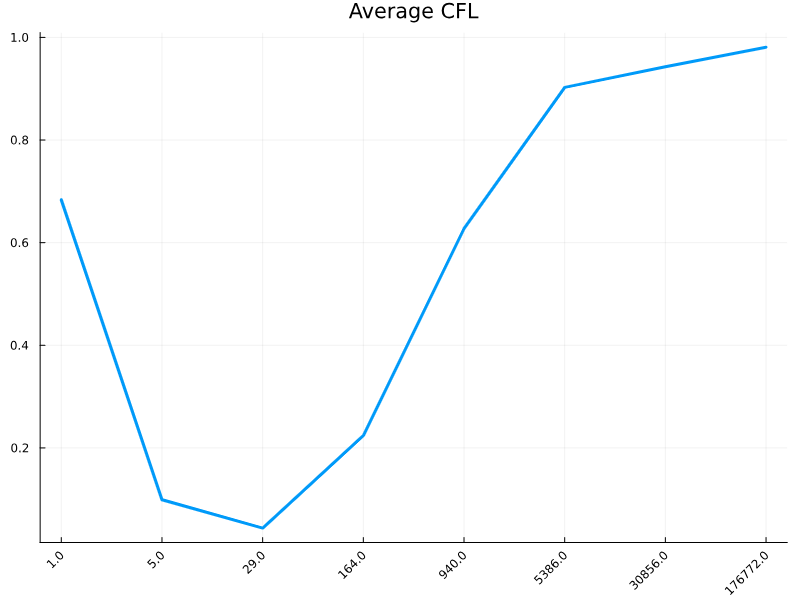
\includegraphics[width=0.65\textwidth]{C:/Users/szjud/OneDrive/Asztali gép/EBCs/CFL-git/Latex codes/Plots/Ushape.png}
    \caption{The U-shape: average reliance on CF-based debt across firm sizes} \label{chart:Ushape}
\end{figure}

\noindent Finally, consider the histogram of CF-reliances. One notable limitation of previous models is that they are unable to reproduce CF-reliance that is between zero and one. My model allows firms to choose any $\tau \in [0,1]$. This could be an nice innovation, but as figure \ref{chart:histog} shows, most firms still prefer to a CF-reliance relatively few firms choose CF-reliance between zero and one. \textit{I went out of my way to achieve this result, but I am not sure if it is worth it.}

\begin{figure}[H]  % [h] indicates placing the image here
    \centering
    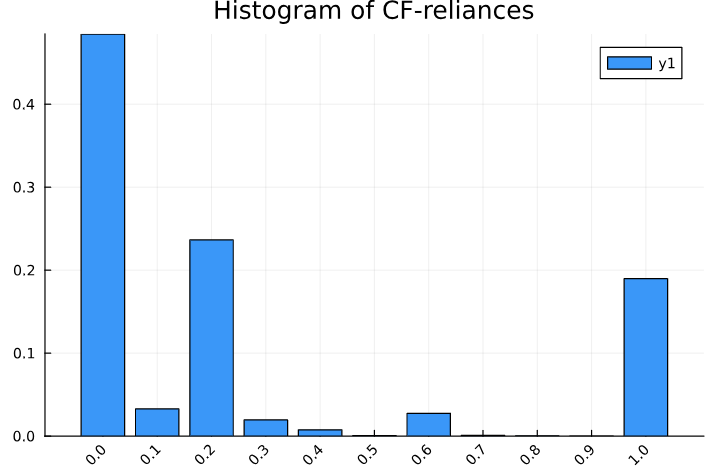
\includegraphics[width=0.8\textwidth]{C:/Users/szjud/OneDrive/Asztali gép/EBCs/CFL-git/Latex codes/Plots/histog.png}
    \caption{The histogram for CF-reliances} \label{chart:histog}
\end{figure}


\newpage

\appendix
\section{Model Solution \label{sec: qualitative analysis}}

In the structural model discussed above, optimal firm policies and the interest rate schedule offered by the lender are jointly determined. That is, lenders set interest rates based on firm policies, but firms choose these policies in light of the interest rate schedule offered to them. This presents a computational issue specific to this model setup. To address this, I adopt the following solution algorithm:\footnote{I similar algorithm is adopted by Corbae and D'Erasmo (2021).}
\begin{enumerate}
    \item Set $q^0$, the starting interest rate equal to $\beta$ for all firm policies and calculate the value of the firm, $V_{cont}(x,\varepsilon)$, the optimal firm policies $k', b', \tau'$ as well as the exit and liquidation policies. 
    \item Calculate the following: the probability of default $P_D$, the probability of liquidation in default $\gamma$, the liquidation value; $\phi_A (1-\delta) k'$ and the reorganization value; $\phi_c V (x', \varepsilon')$ given $q^0$, for each state and firm policy pair
    \item Update interest rate associated with the state-action pair, taking into account the default and liquidation probability and lenders in-default payoffs. This gives  $q^1$. 
    \item Repeat $1-3$ until the optimal policies and interest rates do not change - that is, $ (k^{i},b^{i},\chi_d^{i},q^{i}, V^{i}) = (k^{i-1},b^{i-1},\chi_d^{i-1}, q^{i-1}, V^{i-1}) $.
\end{enumerate}
This algorithm is relatively robust, but it comes at a great computational cost. It usually takes around 30 to 50 iterations to converge, which implies the same number separate solutions of the firm optimization (step number 1) and updating the interests rate schedule (step number 2 and 3). To keep this computational demand manageable, I attempt keep the model as simple as possible in every other respect.

\section{Fixed Costs CF-based Lending \label{sec:fixed costs}}
In section \ref{sec:Default Resolution}, I adopt a highly stylized description of fixed costs: fixed costs of reorganization are imposed only on households which allows me to match the high liquidation probability associated with small corporations. In the interest of keeping the model simple, I do not impose a separate fixed costs on lenders. In practice however, this involves a lengthy negotiation between debtors, creditors, and courts, which imposes significant costs on every involved parties. Hence, when in-default payments are expected through reorganization, the lender must take into account the legal, personnel and time expenses of this process. \vspace{3mm} \\
However, maintaining a cash flow-based debt contract may impose significant costs on the lender even in the normal course of business. Asset-based contracts only require occasional audits of the borrower's assets. In contrast, cash flow-based contracts necessitate that the lender carries out its `due diligence' on an ongoing basis. The apparatus to maintain this monitoring activity may impose significant expenses on creditors.\footnote{This type of cost shares some similarities with the costly state verification first proposed by Towsend (1979).} More generally, such costs could be thought of as all additional expenses lenders face on a regular basis, when they deviate from standardized asset-based contracts.
\vspace{3mm} \\
In summary, evidence would also support for imposing additional fixed costs on creditors for lending against future cash flows. In fact, it would be possible to coin the central trade-off of the model in terms of these fixed cost. In this scenario, asset-based debt would provide the benefit of not having to monitor borrower performance and would offer a quick and cost-effective way of retrieve in default payments. Conversely, CF-based contracts would allow to potentially retrieve a share of the continuation value, but it would impose significant fixed costs on the lender. I do not include this mechanism in the model, as it would produce very similar results to the baseline setup. However, it is important to note that these fixed costs may influence lenders to favor one loan type over another.

\section{Bankruptcy Codes and Practices \label{sec:A1}}
\subsection{Key Principles \label{sec:key principles}}
In the following I highlight some of the key principles laid down in the US bankruptcy code. In this discussion, I highlight those that inform the structural model. \vspace{3mm} \\
\textit{a) The decision to reorganize or liquidate initially lies with the debtor, but lenders may be able enforce the conversion of the case.} Bankruptcy codes typically expect the debtor to first file for liquidation or reorganization - hence, the initial decision is in the hand of the debtor. Creditors may apply for the conversion of the case, but this is approved only under special circumstances. Overall, the influence of a single lender over the default resolution is limited. In the model, I assume that the liquidation decision is made by a third party - the household. However, when making the liquidation decision the household does not take into account the lender's payoffs. This reflects the fact that borrowers have more influence on the default resolution process. \vspace{3mm} \\
\textit{b) Reorganizations must comply with the `best-interest-of-creditors' test.} This rule states that no dissenting creditor should be worse off under the proposed reorganization plan than it would be under the liquidation of the debtor. I refer to this principle as a basis to assume that can consistently expect to recover at least the liquidation value of the firm, when the debt contract is asset-based. \vspace{3mm} \\
\textit{c) Special provisions to facilitate reorganization of SMEs}. Bankruptcy codes often attempt to alleviate the reorganization costs for small enterprises.\footnote{The EU directive allows member states to introduce special provisions to speed up and simplify the reorganization process for SMEs. The US bankruptcy code allow SMEs to file for a small business case (11 U.S.C. § 101(51C)) or under subchapter V of the Small Business Reorganization Act (SBRA), both of which are intended to streamline the reorganization process and reduce costs.} This is based on the recognition that these costs are often prohibitive for small corporations. In the model, I consider the effects of this policy by assuming that small firms only have to pay a fraction of the reorganization cost. However, it should be noted that despite of the special provisions in place, SMEs are still far more likely to choose liquidation. This could be interpreted as evidence that fixed costs of reorganization are still significant for small firms. 

\subsection{Common Themes of Bankruptcy Codes}
The US Bankruptcy Code is structured into chapters, each corresponding to a different type of relief for debtors in financial distress. In this paper, I focus on, chapter 7 deals with liquidations and chapter 11 regulates the reorganization process of US corporations. The European Union does not have a single bankruptcy code, but it has been working towards harmonizing insolvency proceedings across member states, based on the understanding that divergent insolvency laws create barriers across member states. As a result, the Harmonisation Directive\footnote{Directive (EU) 2019/1023 of the European Parliament and of the Council of 20 June 2019 on preventive restructuring frameworks, on discharge of debt and disqualifications, and on measures to increase the efficiency of procedures concerning restructuring, insolvency and discharge of debt.}  was published in June 2019, and member states are required to adopt the necessary legislative changes by July 2021 to comply with it. Although it does not completely standardize bankruptcy procedures, the directive outlines several principles that mirror the main features of chapter 7 and 11 of the US bankruptcy code. It represents a valuable piece of evidence for this discussion, as it collects the set of principles that legislators aim to institute in bankruptcy proceedings. \vspace{3mm} \\
Under both frameworks, the debtor is expected to file for insolvency – although creditors may petition the court to initiate bankruptcy proceedings against the debtor, this is not the norm. If the debtor decides to draft a reorganization plan, creditors may form committees and have their claims heard by courts. The European Union has a more debtor-friendly approach, meaning that creditors have less influence over the outcome of the proceedings, whereas the US system places more weight on the interest of the creditors. However, it is often the case that a debtor has numerous creditors, which limits the influence of any individual creditor over the specifics of the bankruptcy proceedings. 
\vspace{3mm} \\
Notably, both bankruptcy frameworks adhere to the `best interest of creditor test'. The EU Directive refers this as ‘best-interest-of-creditors’ test in OJ L 172/27, art. 49; whereas the US bankruptcy code establishes this principle in 11 U.S. Code § 1129. Moreover, they also both provide special provision for small companies to reorganize at a smaller cost. The EU directive allows member states to introduce special provisions to speed up and simplify the reorganization process for SMEs. The US bankruptcy code allow SMEs to file for a small business case (11 U.S.C. § 101(51C)) or under subchapter V of the Small Business Reorganization Act (SBRA), both of which are intended to streamline the reorganization process and reduce costs.



\section{Data appendix \label{sec:A3}}
\subsection{Compustat and Capital IQ}
Compustat is a comprehensive, financial database maintained by S\&P Global. It offers standardized firm-level information on publicly traded companies compiled from financial statements, regulatory filings and other financial reports. I use the quarterly tables in Compustat North America and drop firms that are not headquartered in the US. Moreover, I exclude financial corporations (SIC code 6000 to 6799) and utility providers (SIC code 4900-4999). \vspace{3mm} \\
S\&P Capital IQ offers an extensive array of debt-level statistics. The two datasets can be connected via the unique firm a identifier (GVKEY), moreover Capital IQ covers most of the Compustat firms and yields consistent firm-level debt data after the aggregation of debt contracts. Although Capital IQ covers most major economies, I only focus on North American corporations, due to limitations introduced by Compustat.  \vspace{3mm} \\
Although both datasets provide high quality reports, reporting differences necessitate some manipulation of the data. Since monetary variables are often reported in the native currency, I bring all observations to USD. Moreover, Capital IQ reports data points in different units (units, thousands or millions). To be consistent to Compustat, I bring all observations to millions of units. It must also be ensured that each observation is uniquely identified by the combination of year, quarter, and debt ID. This may be violated for various reasons, for instance, debt facilities are often reported twice (once with the total accessible debt and once with the currently outstanding amount). Moreover, subsidiaries are also often included in the data. I exclude these to maintain observations at the highest consolidation level. \vspace{3mm} \\
In some instances, debt contracts go missing only to reappear a few quarters later. If this gap between observations is no more the 4 quarters, I use linear interpolation to fill up the data. These cases are relatively rare, they only amount to approximately 7\% of the total sample. To ensure the alignment of consistent observations, I aggregate debt-level data from CapitalIQ to the firm level and cross-reference it with the debt information reported by Compustat. I drop any observations where there is a disparity of more than 20\% between the two datasets. This discards around 8\% of the original sample. Tables \ref{tab:COMPS} and \ref{tab:CAPIQ} summarize Compustat and Capital IQ variables, including their original names and definitions in these datasets.

\begin{table}[htbp]    
\centering
\caption{Compustat variable definitions}
\label{tab:COMPS}
\renewcommand{\arraystretch}{1.5} % Increase the vertical spacing of rows
\resizebox{\textwidth}{!}{%
\begin{tabular}{lp{5cm}p{7cm}} 
\toprule
Variable & Compustat Definition & Description \\
\midrule
Total debt & dlcq+dlttq & Long-Term Debt + Debt in Current Liabilities \\
Leverage & (dlcq+dlttq)/atq & Total debt / Total Assets \\
Collateral & ppentq+invtq+rectq & Total Property, Plant and Equipment (net) + Receivables + Inventory \\
Pledgeability & (ppentq+invtq+rectq)/atq & Collateral / Total Assets \\
Interest coverage & oibdpq / xintq & Operating income before depreciation / Interest related expenses \\
Investment & capxq-sppeq & Capital expenditures - Sale of Property \\
Investment rate & (capxy - sppey) / l.ppegtq & Investment / Lag of Total Property, Plant and Equipment (gross) \\
Equity & atq-ltq & Total assets / Total liabilities \\
Net debt & dlcq+dltq-chq & Total debt - Cash Holdings \\
Liquidity & chq/atq & Cash Holdings / Total Assets \\
Assets & atq & Total Assets (book value) \\
Liabilities & ltq & Liabilities (book value) \\
Revenue & revtq & Total quarter revenue \\
Employees & emp & Total number of employees (thousands) \\
Industry spec. & sic & SIC code \\
Credit rating & spcsrc & S\&P credit rating \\
Added value & revtq - cogsq & Total revenue - Input costs \\
Productivity & $\frac{revtq - cogsq}{ppegtq^{1/3} + emp^{2/3}}$ & Added value / Assets and Employees \\
Age & defined from Capital IQ & Current year - Year founded + 1 \\
\bottomrule
\end{tabular}
}
\end{table}

\newpage

\begin{table}[htbp]    

\centering
\caption{Capital IQ Variables}
\label{tab:CAPIQ}
\begin{tabular}{ll}
\toprule
Variable & Capital IQ \\
\midrule
Loan value & dataitemvalue \\
Decimal of the value & unittypeId \\
Currency of issuance & issuedCurrencyId \vspace{3mm} \\
\multicolumn{2}{l}{\textbf{Used for classification}} \\
Description of the contract & capitalstructuredescription \\
Type of the debt contract & capitalstructuresubtypeid \\
Debt description in text & descriptiontext \\
Secured dummy & securedtypeid \\
Seniority & leveltypeid \vspace{3mm} \\
\multicolumn{2}{l}{\textbf{Firm-level aggregated variables}} \\
Total debt value & Sum of all contracts value \\
AB value & Sum of all AB debt \\
CF value & Sum of all CF debt \\
CF share & CF value / Total debt \\
\bottomrule
\end{tabular}
\end{table}

\section{Additional Figures}

\noindent In line with the previous findings of Lian and Ma (2021) and Öztürk (2022), the total outstanding debt volume that can be classified as CF-based is relatively stable around 75\%. However, starting from 2019, this share drops significantly - from 79\% in 2018Q4 to 71\% 2019Q4 - and it does not fully recover until the end of the sample. It is not clear what causes this abrupt shift in aggregate CFL reliance. Unfortunately, I cannot compare with previous studies because they do not investigate this time period. One explanation could be the Covid-induced economic crisis. However, this leaves the initial drop. which happen before the pandemic had a substantial impact on North American economies unexplained. 

\begin{figure}[H]  % [h] indicates placing the image here
    \centering
    \caption{The share of cash flow-based debt to total debt} \label{chart:CFLshare}
    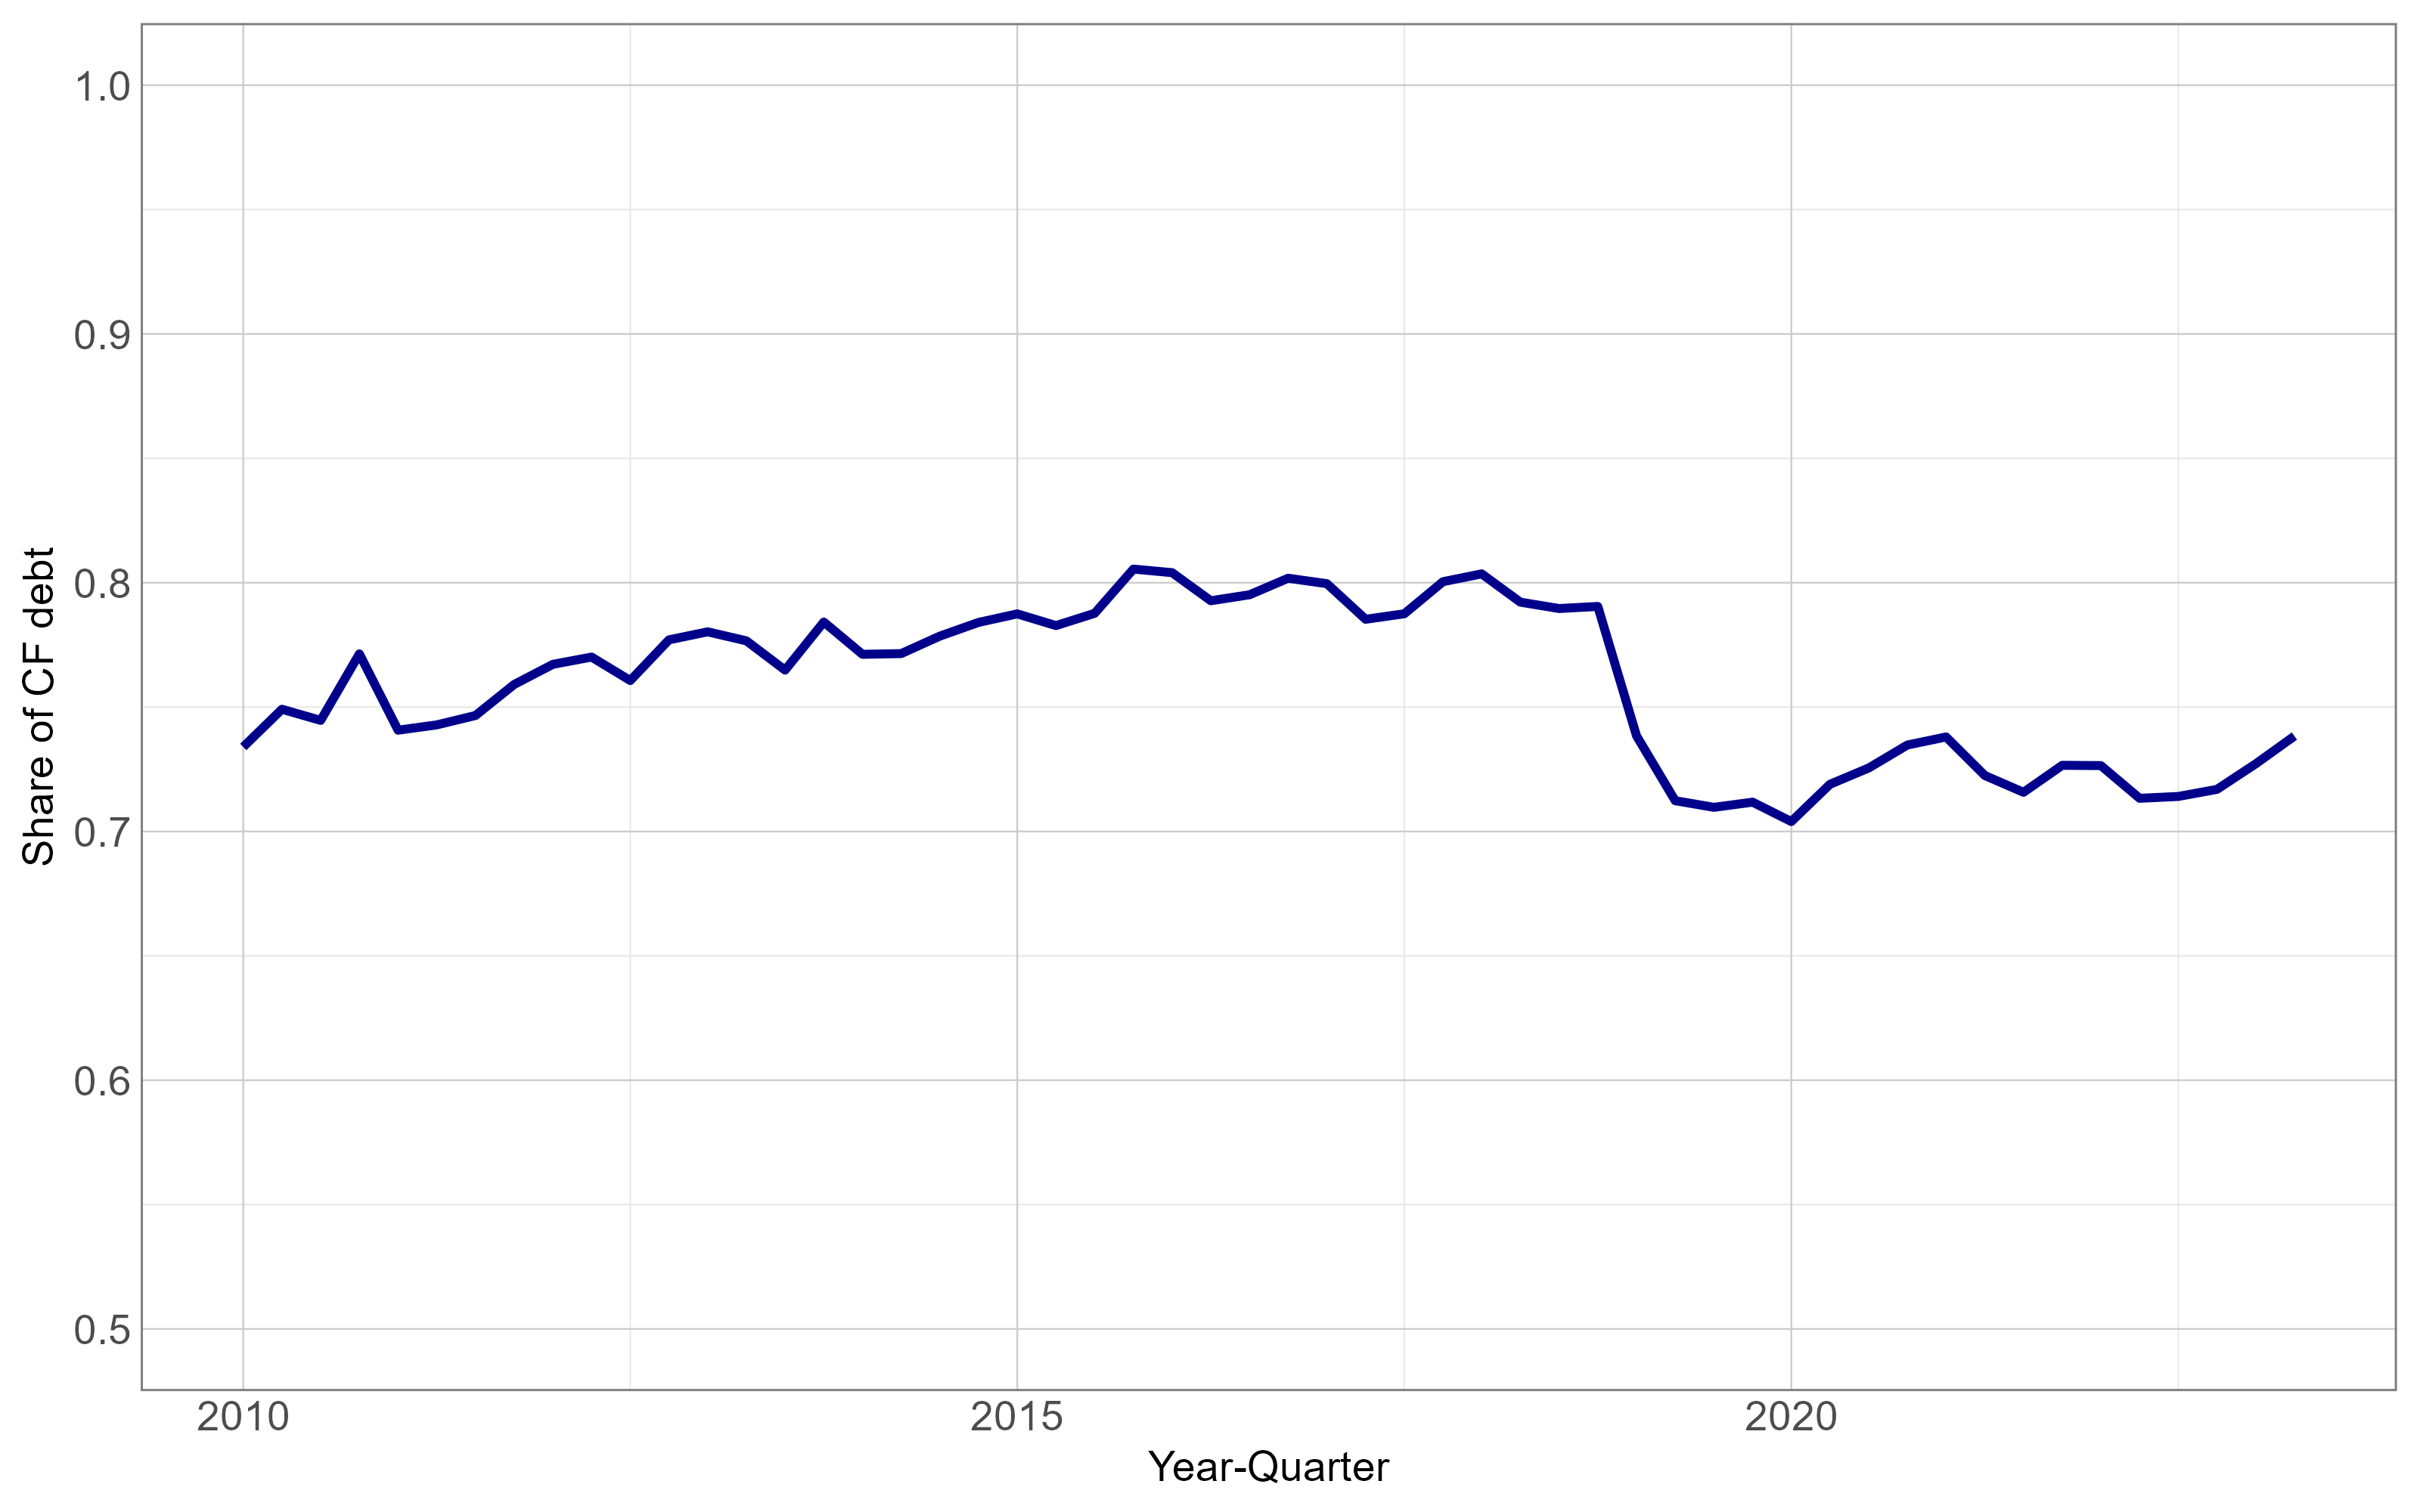
\includegraphics[width=0.7\textwidth]{C:/Users/szjud/OneDrive/Asztali gép/EBCs/CFL-git/Latex codes/Plots/CFshare.png} \\
     \small The share CFL debt to total debt, by volume between 2010Q1 and 2023Q3
\end{figure}

\noindent The figure below shows a stylized graph of the exit - default - continuation decisions of firms. 
\begin{figure}[H]  % [h] indicates placing the image here
    \centering
    \caption{The liquidation decision} \label{chart:DEC}
    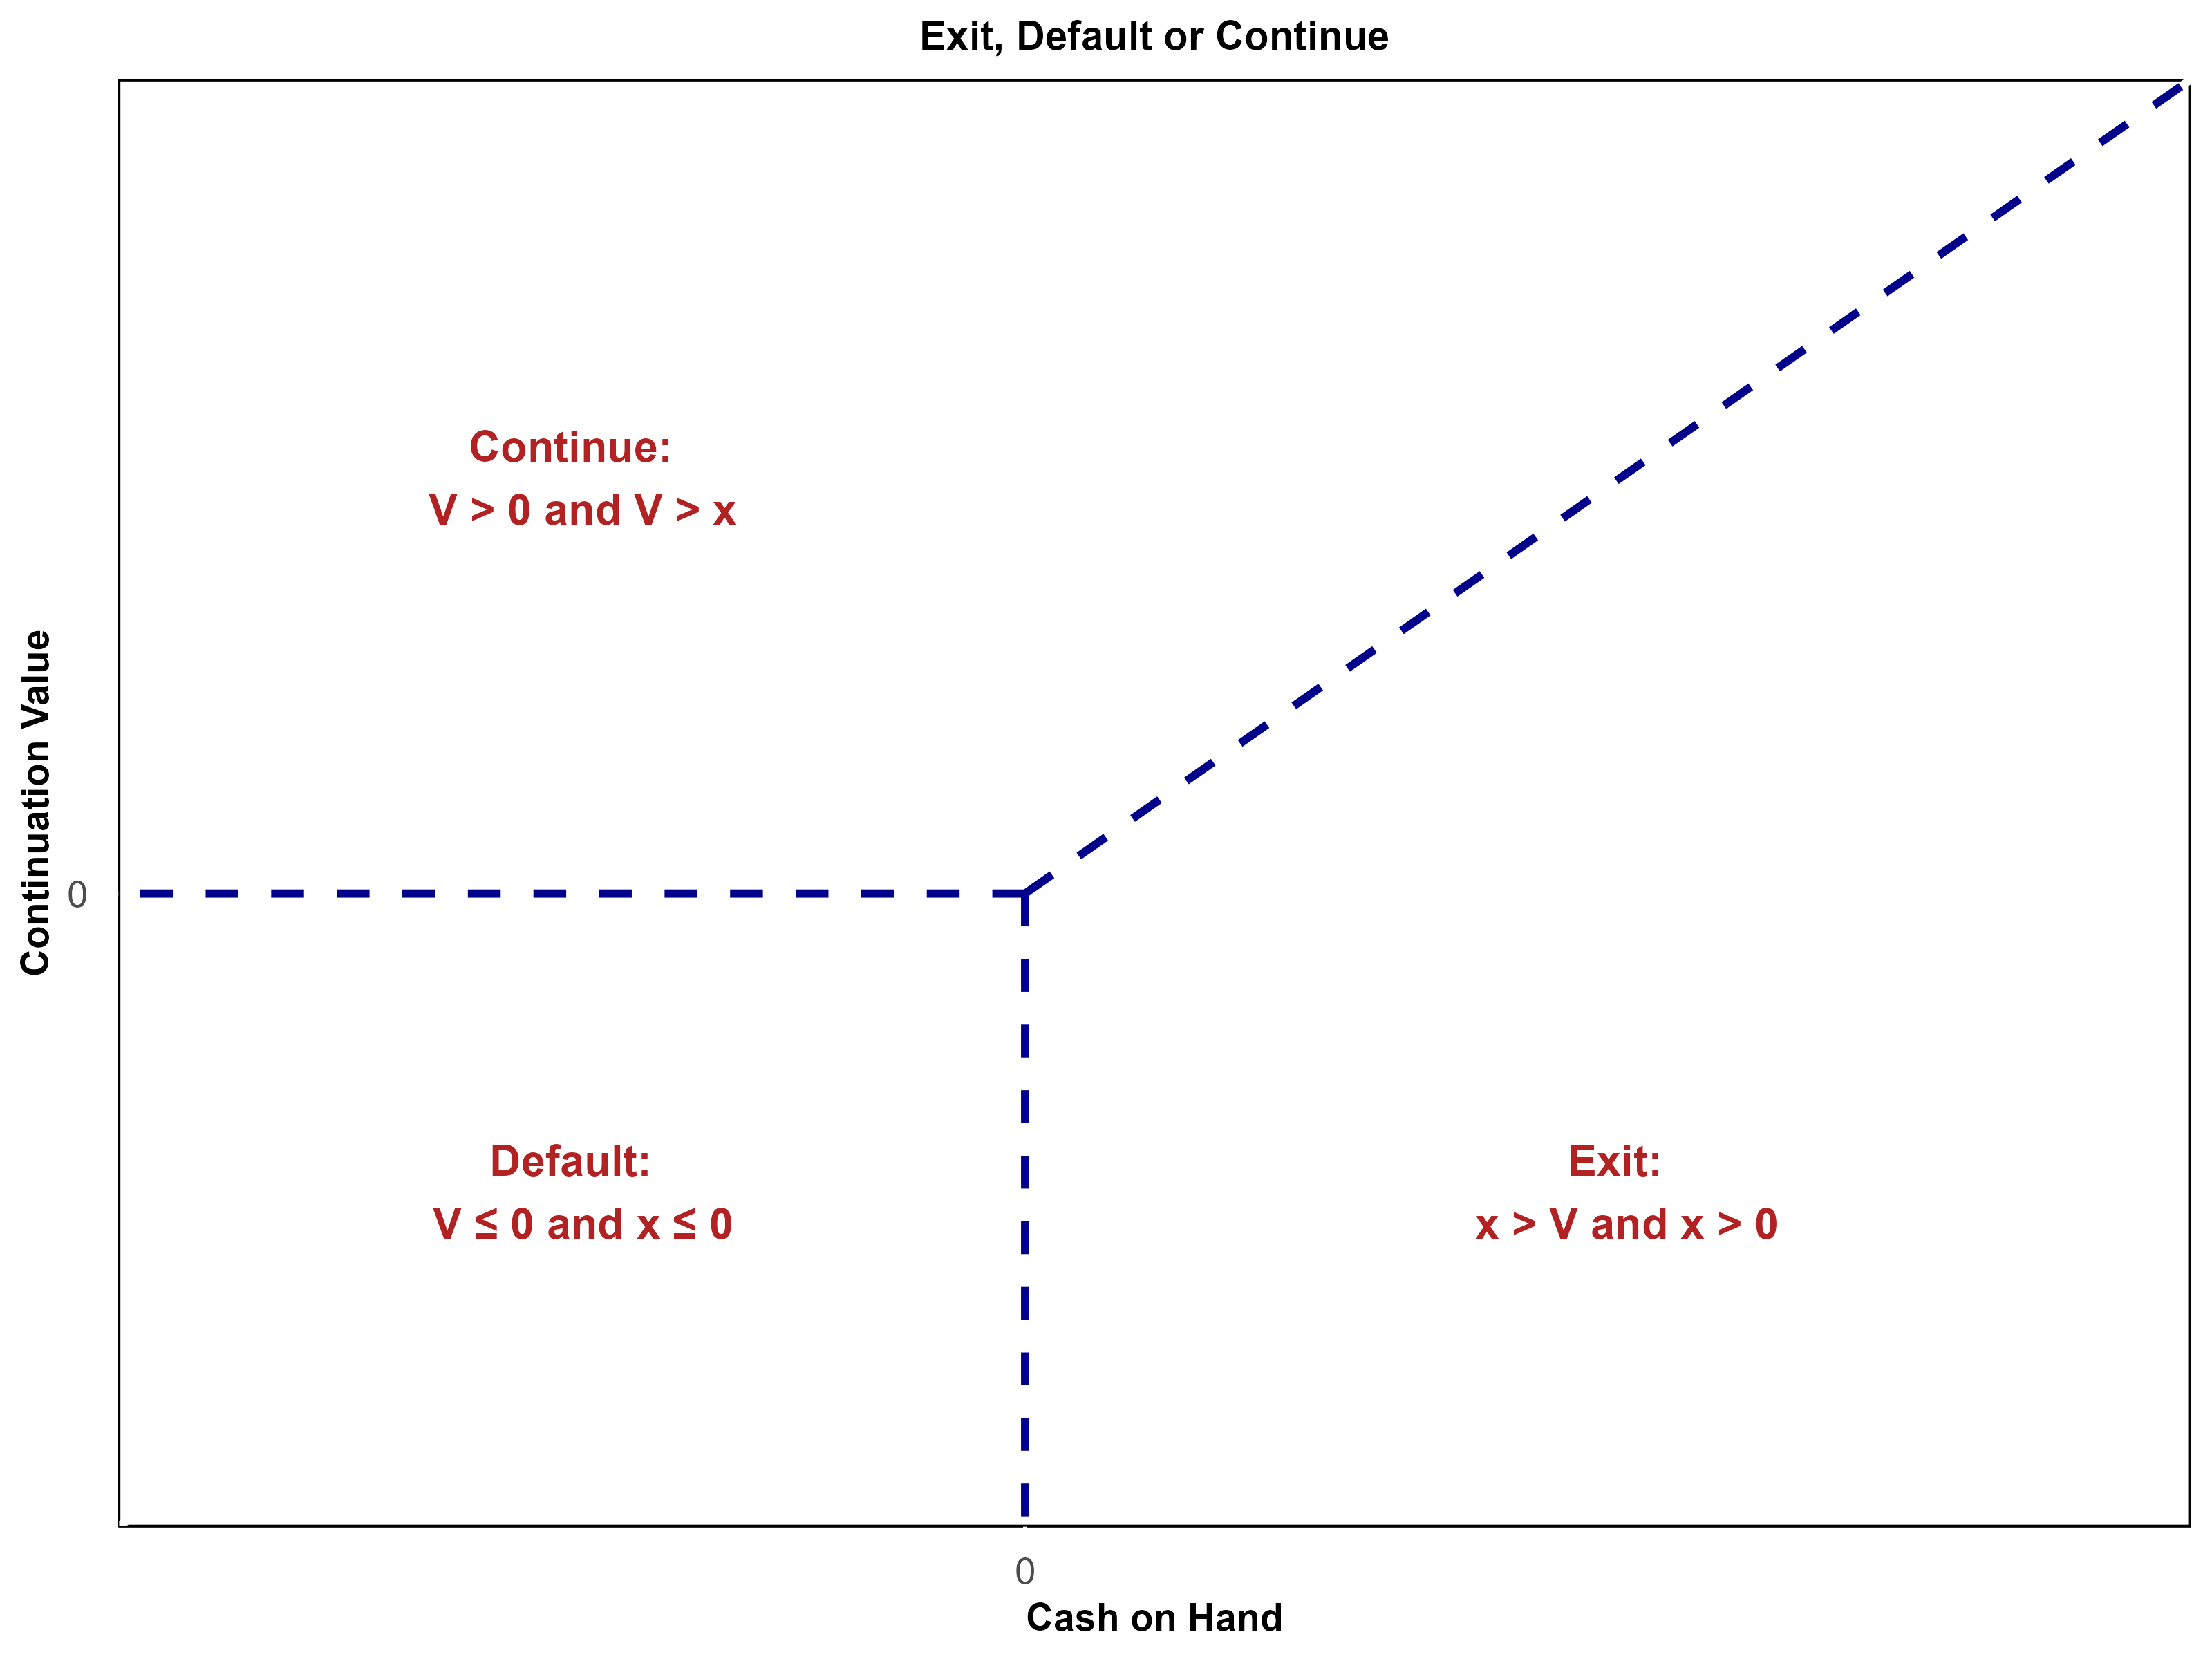
\includegraphics[width=0.7\textwidth]{C:/Users/szjud/OneDrive/Asztali gép/EBCs/CFL-git/Latex codes/Plots/dec.png}
\end{figure}

\end{document}